%%%%%%%%%%%%%
%Clinciu Andrei
%%%%%%%%%%%%%
%%%%%%%%%%%%%
% Preamble 
%%%%%%%%%%%%%

\documentclass[a4paper,11pt,twosided]{book}

%%%%%%%%%%%%%
% Packages
%%%%%%%%%%%%%
\usepackage[english]{babel}
%CHecks syntax only, no dvi produced
%\usepackage{syntonly}
\usepackage[pdftex,bookmarks=true]{hyperref}
\usepackage{cite}
%\usepackage{biblatex}
\usepackage{graphicx,color,colortbl}
\usepackage[usenames,dvipsnames]{xcolor}
\usepackage[small,bf,hang]{caption} 
\usepackage{capt-of}
\usepackage[acronym]{glossaries} % remove the [toc] so it won't show in TOC
%\usepackage{acronym}
%Use this package to make indexes for the used words..
\usepackage{makeidx}
%\usepackage{showidx}
%Use fancy headers..
\usepackage{fancyhdr}
\usepackage{listings} %use new listings 
\usepackage{booktabs}
\usepackage{wrapfig}
\usepackage[toc,page,title,titletoc]{appendix}

%\usepackage{url}
\usepackage{wrapfig} % fig wrapping
%\usepackage{rotating}
%to view any information about any package type
%texdoc <package> - and it will open a pdf
\usepackage[top=2.5cm, bottom=2.5cm, left=3cm, right=2.5cm]{geometry}%make the page a little bigger...
%\usepackage[cm]{fullpage} %standardized margins 
\usepackage{verbatim} %multiline comments..
\usepackage{parskip} % this package places a newline after each paragraph..
\usepackage{tocloft}%toc identing
\usepackage{pdfpages}
%using other fonts
\usepackage{lmodern}
\usepackage[T1]{fontenc}
\usepackage{textcomp}


%%%%%%%%%%%%%
% Define some things
%%%%%%%%%%%%%
\definecolor{myLightGreen}{rgb}{0.58,0.776,0}
\definecolor{listingColor}{HTML}{EEEEFF}
\definecolor{rowhighlight}{HTML}{DFF7AD}
%graphics path
\graphicspath{{images/}}

%Give sections colours
\usepackage{titlesec}

%\titleformat{\section}
%{\normalfont\Large\bfseries}
%{\thesection}{1em}{}
%\color{LimeGreen}\normalfont\Large\bfseries}
%{\color{LimeGreen}\thesection}{1em}{}

\titleformat*{\section}{\normalfont\LARGE\bfseries\color{LimeGreen}}
\titleformat*{\subsection}{\normalfont\Large\bfseries\color{LimeGreen}}
\titleformat*{\subsubsection}{\normalfont\large\bfseries\color{LimeGreen}}

%Enable indexing
%\addcontentsline{toc}{chapter}{Index}
\makeindex{}
\clearpage{}

\setcounter{secnumdepth}{4}%set the counting mechanism on for paragraph & subparagraph
\setcounter{tocdepth}{3}%only allow to 1.2.3 listings.. change to 4 if you want to include subparagraphs in index

%%%%%%%%%%%%%
% Functions
%%%%%%%%%%%%%
% Command to add images. Usage:
% \img[H]{width=5cm}{filename}{caption}
\newcommand{\img}[4][!ht]{                  % The first argument is default 'ht'.
    \begin{figure}[#1]
		\begin{center}
            \includegraphics[#2]{#3}
            \caption{#4\label{#3}}
        \end{center}
    \end{figure}

}

%Fixes the paragraph problems
\newcommand{\myparagraph}[1]{\paragraph{#1}\mbox{}\\}
% Code listings

\lstnewenvironment{codelisting}{
    \vspace{1.2ex plus 0.5ex minus 0.5ex}
    \lstset{
        basicstyle=\small,
        numbers=left,
        numberstyle=\tiny,
        stepnumber=1,
        numbersep=5pt,
        showspaces=false, 
        showstringspaces=false,
        showtabs=false,
        frame=tb,
        tabsize=4,
        captionpos=b,
        breaklines=true,
        breakatwhitespace=false,
	   backgroundcolor=\color{listingColor},
	   belowskip=0pt,
        }
	}
{\vspace{0.9ex plus 0.5ex minus 0.5ex}}

% \codeblock{text}{caption}


\newcommand{\HRule}{\rule{\linewidth}{0.5mm}}
%%%%%%%%%%%%%
% Configuration options
%%%%%%%%%%%%%
%Set hyperlinks to be black..
\hypersetup{colorlinks,%
citecolor=red,%
filecolor=black,%
linkcolor=black,%
urlcolor=blue,%
pdftex,
pdfauthor={Clinciu Andrei},
}
%pdftitle={Hello there friend!}
 % This command is roughly equivalent to \clearpage \input{filename} \clearpage.


%%%%%%%%%%%%%
% Information
%%%%%%%%%%%%%
\author{Clinciu Andrei George}
\title{Internship}

\begin{document}
%\maketitle{}
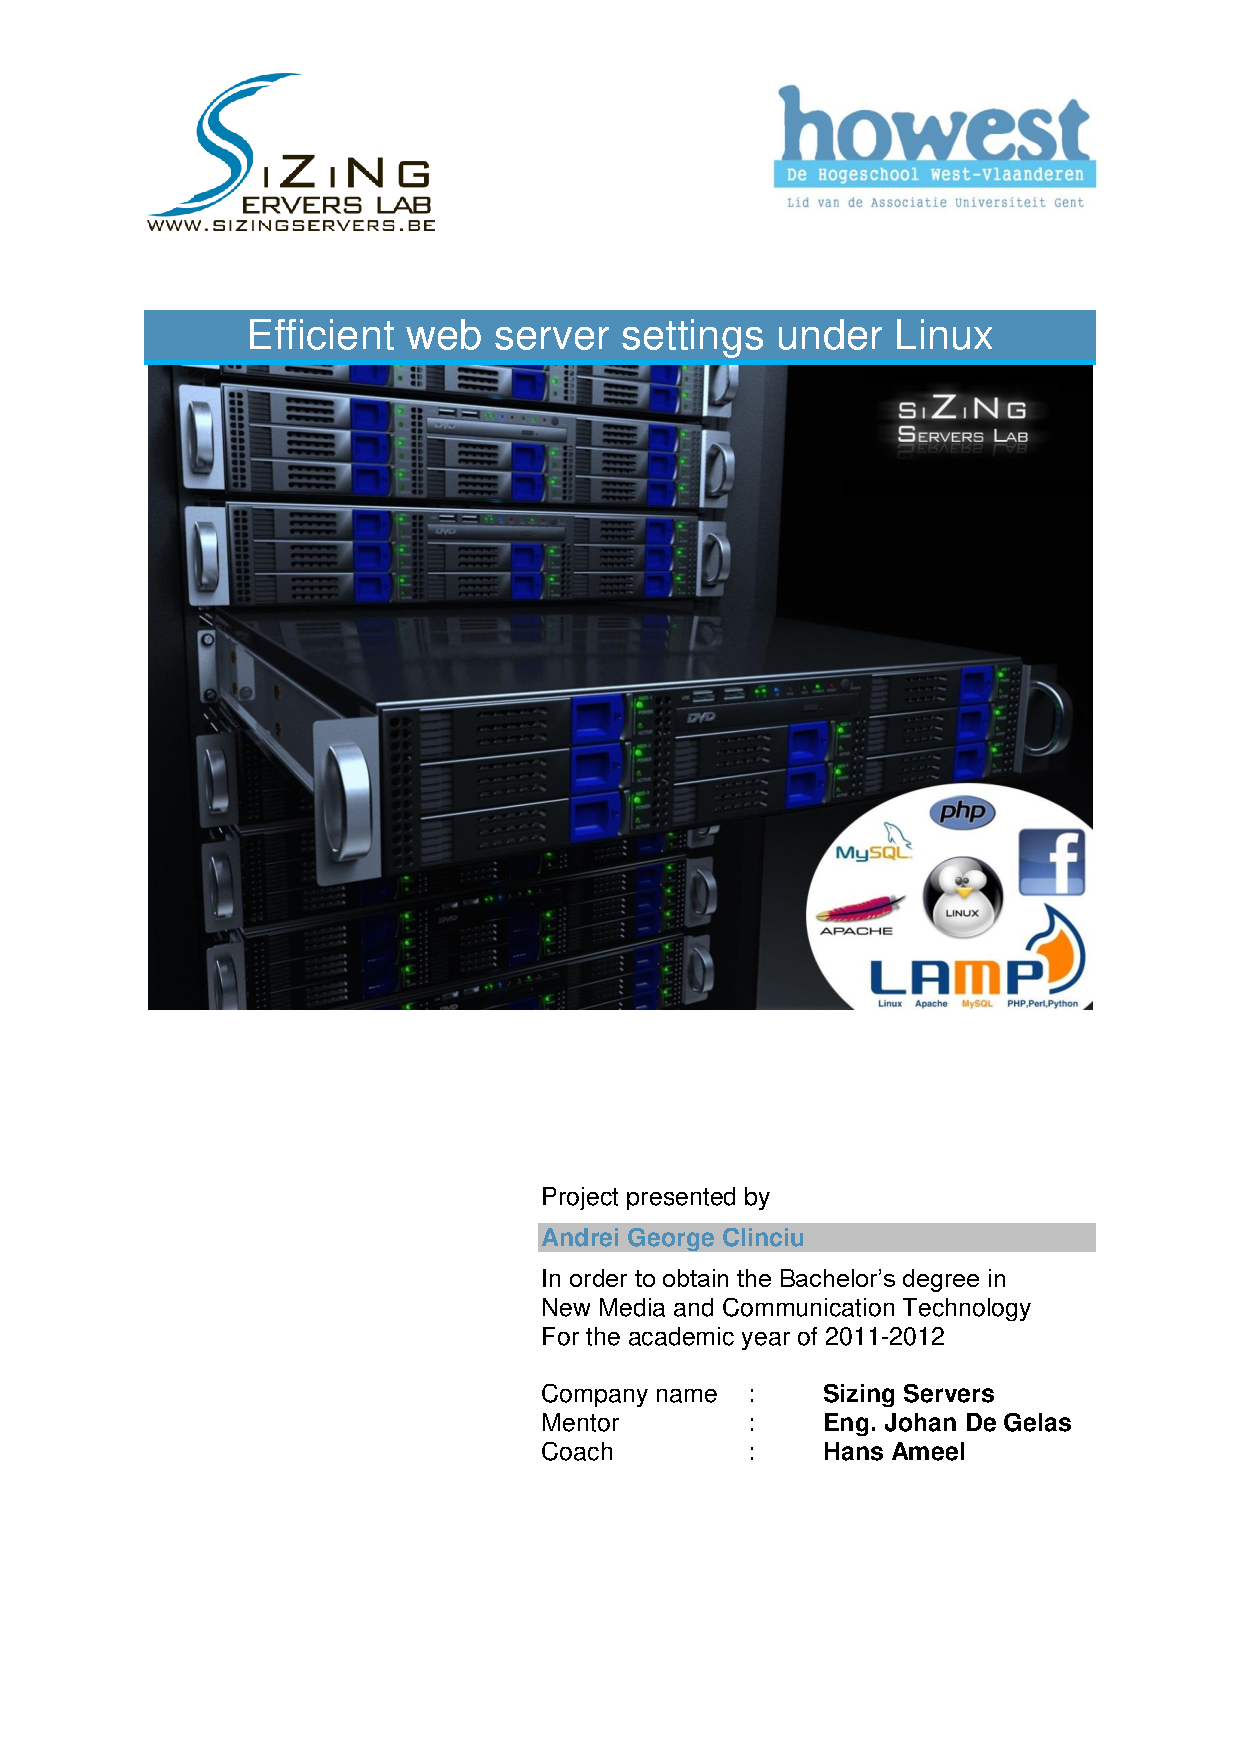
\includepdf[pages={1}]{frontpage_en.pdf}
%% The first page and it must contain at least
%The title, information about it aka the abstract
%student name
%internship coach
%internship mentor
%internship helpers
%where the internship took place + logo of internship
%Howest information + logo
%year it took place
\begin{titlepage}

\begin{quote}
,,Perfection (in design) is achieved not when there is nothing more
to add, but rather when there is nothing more to take away.''

-- Antoine de Saint-Exupéry
\end{quote}

\includegraphics{rId10.jpg}   

\includegraphics[scale=0.25]{sizing-servers-logo.png}   

\textsc{\Large Final year project for obtaining the degree of Bachelor of New Media and Communication Technology}\\[0.5cm]
% Title
\HRule \\[0.4cm]
{ \huge \bfseries Efficient web server settings under Linux}\\[0.7cm]
\HRule \\[1.5cm]

% Author and supervisor
\begin{minipage}{0.4\textwidth}
\begin{flushright} \large{}
%\parident 10px
\emph{Author:}\\
\emph{Internship:} \\
\emph{Internship superviser:} \\
\emph{Internship mentor:} \\
\emph{Academic year:}\\
\end{flushright}
\end{minipage}
\unskip{   }
\begin{minipage}{0.7\textwidth}
\begin{flushleft}
Andrei George \textsc{Clinciu}\\
Sizing Servers Lab\\
Johan  \textsc{De Gelas}\\
Hans  \textsc{Ameel}\\
2011-2012
\end{flushleft}
\end{minipage}

\end{titlepage}

\pagestyle{empty}%remove the numbering.. etc
\thispagestyle{empty}

%\appendix{}

%The sections before the table of contents

\clearpage{}
\section*{Foreword}
My name is Andrei Clinciu and I'm a student in my final year following NMCT(New Media and Communication Technology) at Howest.
In my last year I've chosen majors like operating systems, network infrastructure, information systems security, virtualisation and cloud computing.
I enjoy programming a lot and want to combine it with the Linux operating system.

Throughout the existence of the Web there were always developers who wanted to create dynamic content to attract more people to their websites.
Within this evolution dynamic languages into the context. 

As the Internet did not have that many users in the beginning you could notice lagging websites but didn't have a faster connection so everything was all right.
With the evolution of better network connections and the wide spread of computers, videos, images and advanced web applications many bottlenecks were noticed.

This document explains how to optimise such applications by optimally managing your configuration.
Optimising existing software to gain more throughput and a better response time is a must for today's websites since the cost of electricity grows daily.

This thesis is meant for the researchers at Sizing Servers so they can follow most of the steps here to be able to build upon it and further their work.
It is also meant for people who want to set up their own web server, even people searching for quick speed-up tricks.
Regard it as a work of research with a lot of trial and error. For me this has been very enriching. 

All of the examples here have been set up using Ubuntu Linux 11.10 (server edition).
Any other Linux distribution should work, though there might be some differences. It's best advised to first test everything on Ubuntu.

I'd like to thank everyone from the Sizing Servers team for the possibility to have an internship in my last year at Howest, also for the acceptance and the nice time we had together.
Many thanks to my internship supervisor Johan De Gelas for the project ideas. 
Last but not least my appreciation for Hans Ameel my coach, who reviewed my work and presentation helping me in the technical field and attentive analysing my linguistic mistakes.

I'm sure that you, the reader, will find something interesting  in this work.

With regards
\\Andrei Clinciu.

\clearpage{}
\section*{Summary}
This work of research is about software optimisations or configuration settings that can make your software work better and require less CPU power. 
Thus enabling servers to do their calculations faster and use less energy. 

The problem is not how to begin or what to do because there is enough information on that but how to notice when something isn't productive.
Only continuing if the results are optimal.
This is a big problem since in research you can waste years of intensive work to just find out that it was not worth researching in the first place.

The best way to be sure that you won't fail so fast is to document everything you do as much as possible. 
That's what I've done from the beginning. Gathering information and reviewing existing tests that have something to do with the research I'm working on to see if it's a good idea. 
For the full results of each phase look at the end of each section.

The usage of Intel Energy Checker and how to integrate it in your software to be able to see how much energy an application uses is explained in \autoref{sec:IntelSDK} on page \pageref{sec:IntelSDK}.
It's very hard to integrate it into an existing project. The network agent it uses isn't usable for what we required. 

A detailed mini documentation on how to use the HipHop  compiler for PHP made by Facebook is found at \autoref{sec:using_hiphop} on page \pageref{sec:using_hiphop}. What it is, how it can be used, what the speed benefits are. 
The conclusion is that HipHop can't be used in a production environment because  any existing website needs to be rewritten following some guidelines 
and that it takes a long time to compile. If you do compile it without problems, you'll notice that every change requires a recompilation of everything which is not so efficient. 
Only one site may be hosted per binary file and those binary files are 50 mb's.

Ever wanted set up an existing Apache installation on a SSD? If so go to \autoref{sec:lamp_optimise} on page \pageref{sec:lamp_optimise}. There you will find a little introduction on how to setup your SSD and migrate MySQL databases and Apache's PHP files to a SSD for speed benefits. 
Code profiling techniques are likewise explained including Xdebug for PHP.

If you're only interested in LAMP settings to make your LAMP installation work better you can fast forward to \autoref{sec:testcasesphpBB}  on page \pageref{sec:testcasesphpBB}.
There examples and graphics show different settings and how they have an impact on the throughput and response time.
One of the best things you can do to your website is install APC and use the extension in applications. It decreases the CPU usage to half.

For a quick overview of the Plotchart script written in TCL you can always refer to \autoref{sec:scripts}  on page \pageref{sec:scripts}. It imports log data from the stresstests and generates graphics for the CPU, memory usage, disk usage, network traffic and some other related graphics. 
This script has helped me in distinguishing the data without having to spend a whole day in Excel and plotting everything manually.

For the final conclusion you can jump to \autoref{sec:scripts}  on page \pageref{sec:scripts}.

%KEEP IT SIMPLE 
\clearpage{}
%verklarende woordenlijst
%terms + alphabetical
%\setglossarystyle[acronym]{style=long,border=true}
\makeglossaries{}
\newacronym{cobol}{COBOL}{COmmon Business-Oriented Language}
\newacronym{pl}{PL}{Productivity Link}
\newacronym{uuid}{UUID}{Universally Unique Identifier}
\newacronym{tcpip}{TCP/IP}{Transmission Control Protocol over Internet Protocol}
\newacronym{hphp}{HPHP}{HipHop for PHP}
\newacronym{hphpi}{HPHPI}{HipHop for PHP interpreter}
\newacronym{html}{HTML}{HyperText Markup Language}
\newacronym{css}{CSS}{Cascading Style Sheets}
\newacronym{sql}{SQL}{Structured Query Language}
\newacronym{lamp}{LAMP}{Linux, Apache, MySQL and PHP}
\newacronym{cpu}{CPU}{Central Processing Unit}
\newacronym{ram}{RAM}{Random Access Memory}
\newacronym{ssd}{SSD}{Solid State Disk}
\newacronym{tcl}{TCL}{Tool Command Language}
\newacronym{csv}{CSV}{Comma Separated Values}

\newglossaryentry{sqlite}
{
	name={SQLite},
	text={SQLite},
	description={SQLite is a software library that implements a self-contained, serverless, zero-configuration, transactional SQL database engine. SQLite is the most widely deployed SQL database engine in the world. The source code for SQLite is in the public domain.}
}
\newglossaryentry{api}
{
	name={API},
	first={Application Programming Interface (API)},
	text={API},
	description={An application programming interface (API) is a specification intended to be used 
			as an interface by software components to communicate with each other. 
			An API may include specifications for routines, data structures, object classes, and variables
	}
}
\newglossaryentry{sdk}
{
	name={SDK},
	first={Software development kit (SDK)},
	text={SDK},
	description={A software development kit (SDK or "devkit") is typically a set of software development 
		tools that allows for the creation of applications for a certain software package, software framework, 
		hardware platform, computer system, video game console, operating system, or similar platform}
}
\newglossaryentry{ide}
{
	name={IDE},
	first={Integrated development environment (IDE)},
	text={IDE},
	description={An integrated development environment (IDE) is a software application that provides comprehensive 	facilities to computer programmers for software development}
}
\newglossaryentry{php}
{
	name={PHP},
	first={Hypertext Preprocessor (PHP)},
	text={PHP},
	description={PHP is a general-purpose server-side scripting language originally designed for Web development to produce dynamic Web pages}
}
\newglossaryentry{cms}
{
	name={CMS},
	first={Content Management System (CMS)},
	text={CMS},
	description={A content management system (CMS) is a computer system that allows publishing, editing, and modifying content as well as site maintenance from a central page. It provides a collection of procedures used to manage work flow in a collaborative environment.}
}
\newglossaryentry{apache}
{
	name={Apache},
	first={Apache},
	text={Apache},
	description={Apache HTTP Server, commonly referred to as Apache}
}
\newglossaryentry{mysql}
{
	name={MySQL},
	first={MySQL},
	text={MySQL},
	description={
	MySQL is the world's most used relational database management system (RDBMS) that runs as a server providing multi-user access to a number of databases. It is named after developer Michael Widenius' daughter, My. The SQL phrase stands for Structured Query Language}
}
\newglossaryentry{vapus}
{
	name={vApus},
	first={Virtualized Application Unique Stresstesting (vApus)},
	text={vApus},
	description={An advanced Application Stresstesting program.}
}
\newglossaryentry{mime}
{
	name={MIME},
	first={Multipurpose Internet Mail Extensions (MIME)},
	text={MIME},
	description={Multipurpose Internet Mail Extensions (MIME) is an Internet standard that extends the format of email to support   
		Text in character sets other than ASCII, Non-text attachments, 	Message bodies with multiple parts and Header information in non-ASCII character sets
	}
}
\newglossaryentry{raid}
{
	name={RAID},
	first={redundant array of independent disks (RAID)},
	text={RAID},
	description={
	RAID (redundant array of independent disks) is a storage technology that combines multiple disk drive components into a logical unit. Data is distributed across the drives in one of several ways called "RAID levels", depending on what level of redundancy and performance (via parallel communication) is required}
}
\newglossaryentry{apc}
{
	name={APC},
	first={Alternative PHP Cache (APC)},
	text={APC},
	description={The Alternative PHP Cache (APC) is a free and open opcode cache for PHP. Its goal is to provide a free, open, and robust framework for caching and optimizing PHP intermediate code}
}
\newglossaryentry{memcached}
{
	name={Memcached},
	text={Memcached},
	description={Memcached is a high-performance, distributed memory object caching system, generic in nature, but originally intended for use in speeding up dynamic web applications by alleviating database load}
}
\newglossaryentry{hyperthreading}
{
	name={Hyper-Threading},
	text={Hyper-Threading},
	description={Hyper-threading (abbreviated HTT or HT) is Intel's term for its simultaneous multithreading. It works by duplicating certain sections of the processor - those that store the architectural state - but not duplicating the main execution resources}
	}
\newglossaryentry{makefile}
{
	name={Makefile},
	text={\textbf{Makefile}},
	description={In software development, Make is a utility that automatically builds executable programs and libraries from source code by reading files called makefiles which specify how to derive the target program}
}

%\makeacronym
\printglossaries{}
%\printacronym
\clearpage{}

%\section*{Symbols list}
%\clearpage{}

%remove these lines when you want to ident the table of contents:)

\cftsetindents{section}{0.5in}{0.5in}
\cftsetindents{subsection}{0.5in}{0.5in}
\cftsetindents{subsubsection}{0.5in}{0.5in}
\cftsetindents{paragraph}{0.5in}{0.5in}
% insert the table of contents
\tableofcontents{}
\clearpage

\pagestyle{headings}
\section{The lovely world of research}
\subsection{About Sizing Servers lab}
The Sizing Servers Lab is a government subsidized and acknowledged research lab, located in the University College of Western Flanders, 
doing razor sharp research into the newest server technologies, both hardware- and software-wise.
For over 4 years, the lab has offered several companies the opportunity to access this expertise, and thanks to a dynamic and growing team,
Sizing Servers is able to offer highly specialized services to exactly those companies in need of expertise that require a deep and academic understanding of the subject matter.

Over the past few years, the lab has always been just ahead of the industry by diving deep into all the different aspects of virtualization
and their impact on the performance of the server landscape. The results of this research, enhanced by their in-house developed unique stress testing 
software vApus, have already been published to publications read by IT professionals from all over the world, 
and a successful themeday that received the attention of over 100 visitors.

Thanks to the very broad collection of important partners the lab is able to enjoy, it is now capable of putting extensive 
research into the next big wave of innovation: Cloud Computing.
\subsection{Why have I chosen for this internship}
I have chosen for this kind of internship because I knew I could learn a lot and be up to date with the newest software and hardware trends on the market.
Being around people that work with the newest hardware and know a lot about everything on the market is a big plus for learning new things.

\subsection{My research projects}
I didn't know exactly what I was going to do until I first started but even at that moment I did not have a good idea on everything. 
It took a few weeks and finishing a few little researches, reading a lot of documentation to get a  better view on everything.

My job is actually to research how software can perform better in terms of higher throughput and lower response time thus using less energy all the way.
This is done by reading a lot of documentation and testing many of the things myself. 
Documenting what I've found is a must because everything I do might be useful for Sizing Servers in the future so they have a reference whenever they need to re-test something and give them a good starting point.

My first research project was on how to implement Intel Energy Checker into other existing software so we can "measure" the energy usage of that software.
This was somewhat problematic because you require the source of that software and it isn't easy to find and the implementation is almost impossible for real life tests.

My second research project was on HipHop \gls{php} to C++ compiler made by Facebook. This is done so the \gls{cpu} usage is lowered and you get a better workload on the servers.
I had to see how it would be possible to convert an existing \gls{php} website to a HipHop compiled one. Not quite that easy.

My third research project being the longest one was on optimising \gls{lamp}. 
First of all I had to search what bottlenecks are in reality, what optimisations are available.
After this I prepared the system, using \gls{raid} on \gls{ssd}'s for speed so the hard disks wouldn't become the bottleneck. 
This meant the migration of \gls{apache} and \gls{mysql} to the SSD.
Then starting the test from 1 core to the full 16 cores to view how everything would scale.

After the setup was done I had to do research on small things to use so there would be an increase in speed.
Many configuration options are either in \gls{apache} or in \gls{php} of which one of the most important was \gls{apc}.

%%%%%%%%%%%%%
% INCLUDES
%%%%%%%%%%%%%

\pagestyle{fancy}
% with this we ensure that the chapter and section
% headings are in lowercase.
\begin{comment}
\renewcommand{\chaptermark}[1]{%
\markboth{#1}{}}
\renewcommand{\sectionmark}[1]{%
\markright{\thesection\ #1}}
\fancyhf{} % delete current header and footer
\fancyhead[LE,RO]{\bfseries\thepage}
\fancyhead[LO]{\bfseries\rightmark}
\fancyhead[RE]{\bfseries\leftmark}
\renewcommand{\headrulewidth}{0.5pt}
\renewcommand{\footrulewidth}{0pt}
\addtolength{\headheight}{0.5pt} % space for the rule
\fancypagestyle{plain}{%
	\fancyhead{} % get rid of headers on plain pages
	\renewcommand{\headrulewidth}{0pt} % and the line
}
\end{comment}

\section{Intel energy Checker SDK}\label{sec:IntelSDK}
\subsection{Product overview}
``The Intel\textsuperscript{\textregistered} Energy Checker \gls{api} provides the functions required for exporting and importing counters from an application. A counter stores the number of times a particular event or process has occurred, much like the way an odometer records the distance a car has travelled. Other applications can read these counters and take actions based on current counter values or trends derived from reading those counters over time. The core Intel\textsuperscript{\textregistered} Energy Checker \gls{api} consists of five functions to open, re-open, read, write, and close a counter.

The Intel\textsuperscript{\textregistered} Energy Checker \gls{sdk} \gls{api} exposes metrics of "useful work" done by an application through easy software instrumentation. For example, the amount of useful work done by a payroll application is different from the amount of useful work performed by a video serving application, a database application, or a mail server application. All too often, activity is measured by how busy a server is while running an application rather than by how much work that application completes. The Intel\textsuperscript{\textregistered} Energy Checker \gls{sdk} provides a way for the software developer to determine what measures of "useful work" are important for that application and expose those metrics through a simple \gls{api}.''\cite{intel_ec_sdk_website}  
\nolinebreak
\subsubsection{Documentation}
Most of the documentation and examples shown here are based on the \textbf{Intel(R) Energy Checker SDK--User Guide.pdf}\cite{intel_userGuide} examples and documentation. 

The \gls{sdk} includes a few PDF's with information about it. To understand how it works someone needs to read the whole documentation on forehand. A simple demonstration won't prove anything to the reader before he understands what it does exactly. I myself have read the User Guide two times before I could understand what it does and how to use some examples.

Since this is a \gls{sdk} don't expect to know how to use it in a few pages, most people don't know how to use an \gls{ide} or \gls{sdk} even after a few months of usage!
\nolinebreak
\subsubsection{Programs included in SDK}
It's a \gls{sdk} thus it has a lot of little programs that each do something, they don't all work as expected after compilation, some need ROOT access, others need to be edited. It can be expected that while working with engineering and research applications you'll have to tweak a lot of things before they work. It has a broad usage and is very complex.

It can even be used in scripting environments with precompiled functions.
\subsubsection{Basic concepts}
One of the basic concepts is the counters, and it numbers the particular times some event or process occurred. Like the number of kilometres a vehicle had travelled. Those can be exported or imported using the \gls{pl}.\nolinebreak
\myparagraph{Productivity links}
\\An application imports and exports \gls{pl}'s from a standard location through the EC \gls{api}.

"The \gls{api} automatically allows multiple instances of an application to maintain separate counters for each instance of the application." This means you can easily use it in multi-threaded applications.

Each application can simultaneously open 10 \gls{pl}'s and each \gls{pl} can have a maximum of 512 counters, thus 5120 counters in total per application. \gls{pl} counters store ONLY numerical data! The names must be valid and max 199 chars.  The values are usually long integers ($2^{64-}1$ bits).
\myparagraph{Suffix counters}
\\You can use suffix counters to just append a type of suffix. Sign suffix positive changes to negative  and the other way around, these are just files with the same counter.

\textbf{Software Status Counter}
\\It's recommended to define the Status counter to indicate the states of an application. 
\\0 = terminated, 1 = idle, 2 = initializing, 3 = active, 4= terminating.

\textbf{Metrics}
\\Calculate the useful work done by the software and see the energy consumed.

\textbf{API Overview}
\\The \gls{api} code is provided as a set of two C source code files (\textbf{productivity\_link.c} and \textbf{productivity\_link.h}). Therefore, no external libraries or run-time software is required with the instrumented application; this allows Intel EC-instrumented applications to run standalone, without imposing any additional library dependencies. Alternatively, Intel EC code can be built into Dynamic Link Libraries (DLLs) or Shared Objects (SOs) to provide dynamic linkage at runtime.

\textbf{Symbols}
\\Each command and function needs to use a specific symbol. See the Intel R Energy checker SDK  User Guide PDF for more details. This is useful for the building of the library also known as compilation.
\subsubsection{API commands}
The API is very simple, it only uses 5 commands. But to correctly include these commands in your application is the task of the software designer.
\myparagraph{pl\_open()}
This command creates a \gls{pl} and creates the counters specified by couter\_names. Those counters will be used by other functions to store data. The returned value is an integer that can be identified by a special error code at 3.4.6 in the ,,Intel Energy Checker SDK''
%\\(move this to the appendix?)

\textbf{Syntax}
\begin{codelisting}
int pl_open(
	char *application_name,
	unsigned int counter_count,
	const char *counter_names[],
	uuid_t *uuid
);
\end{codelisting}

\textbf{Parameters}
\begin{codelisting}
application_name 	Pointer to a zero terminated ASCII string
counter_count 		Number of  counters to create
counter_names 		Array of pointers to zero terminated ASCII strings
uuid				Pointer to a uuid
\end{codelisting}
\myparagraph{pl\_close()}
This command closes a previously opened \gls{pl}, it also frees the memory used.\nolinebreak
\begin{codelisting}
int pl_close(
	int pl_descriptor
);
\end{codelisting}
\myparagraph{pl\_write()}
This simple command writes values into \gls{pl} counters. You can use a write action for every counter.\nolinebreak

\textbf{Syntax}
\begin{codelisting}
int pl_write(
	int pl_descriptor,
	const void *pointer_to_data,
	unsigned int counter_offset
);
\end{codelisting}

\textbf{Parameters}
\begin{codelisting}
pl_descriptor 	A valid Productivity Link descriptor.
pointer_to_data	A valid pointer to a memory location storing an unsigned long long value.
counter_offset	A valid index in the PL's counters list (zero-relative).
\end{codelisting}
\myparagraph{pl\_read()}
This command is analogous to the write one, it reads the information. The pointer to the data must be large enough to hold the data.

\textbf{Syntax}
\begin{codelisting}
int pl_read(
	int pl_descriptor,
	const void *ponter_to_data,
	unsigned int counter_offset
);
\end{codelisting}
\myparagraph{pl\_attach()}
Sometimes it's a good idea to attach to an existing pl configuration file to read or edit it.

\textbf{Syntax}
\begin{codelisting}
int pl_attach (
	char *pl_config_ini_file_name
);
\end{codelisting}
Please refer to the Appendix \ref{hellotest.c} (p. \pageref{hellotest.c}) \textbf{hellotest.c} for a working example.

\subsection{File system-less mode}
The \gls{api} gives the option to use a system-less mode for devices like mobile phones etc. It stores the \gls{pl} information on an agent via the \gls{tcpip} network.

To do so define \textbf{\_\_PL\_FILESYSTEM\_LESS\_\_} in your code while building the application. The Agents are the servers. 
A sample agent is included as an example in the \gls{sdk}; \textbf{productivity\_link\_agent.c}. It can help for further development.
\subsubsection{PL protocol}
The PL protocol is a simple network protocol designed to encapsulate and send \gls{api} calls to a networked agent, and to receive and decode a networked agent's answer to the \gls{api} calls. The application sees the same information between the file-system-based and the system-less mode. 

The encoding of each function is explained in the documentation, and it's fairly technical maybe the agent can be used to just store the files on another system and nothing more. See more info at the \gls{pl} Agent!
\subsubsection{Network Configuration}
When compiled in file system-less mode, the \gls{api} uses two environment variables to specify the IPV4 address and port number in order to communicate with an agent.

The IPV4 address environment variable is PL\_AGENT\_ADDRESS. If the variable does not exist, then PL\_DEFAULT\_PL\_AGENT\_ADDRESS (127.0.0.1)  is used.

The port number environment variable is PL\_AGENT\_PL\_PORT. If it does not exist, then PL\_DEFAULT\_PL\_AGENT\_PL\_PORT (49253)  is used.
\subsection{Using ESRV and TSRV Data}
\subsubsection{Compilation in Geany}
Compiling an application could be done by using either the \gls{makefile} provided for the default applications or using a custom command from the \gls{makefile} and add it to Geany so it's easier to edit and compile your own files. For multiple files or a bigger project it's suggested to just edit the \gls{makefile} as you like.

Sample compilation for Linux:
\begin{codelisting}
	/usr/bin/gcc -D__PL_LINUX__ -D__PL_GENERATE_INI__ -D__PL_GENERATE_INI_VERSION_TAGGING__ -D__PL_GENERATE_INI_BUILD_TAGGING__ -D__PL_GENERATE_INI_DATE_AND_TIME_TAGGING__ -D__PL_BLOCKING_COUNTER_FILE_LOCK__ -D__PL_EXTRA_INPUT_CHECKS__ -m64  -O2 -msse -Wall -fPIC -std=gnu99 -D_SVID_SOURCE -D_REENTRANT -D_LIBC_REENTRANT -pthread	-I"/home/lostone/School/3nmct/Stage - Sizing Servers/iecsdk"/src/core_api "%f" "/home/lostone/School/3nmct/Stage - Sizing Servers/iecsdk"/src/core_api/productivity_link.c 	-o "%e" 	-lpthread -luuid -ldl
\end{codelisting}
\subsubsection{Start ESRV (Energy server)}
I eventually had enough good luck to successfully start the ESRV energy server. This server uses either a simulated device or a real device to measure the energy usage and log all the counters. But be sure to compile the energy ESRV driver kits from \textbf{/iecsdk/utils/device\_driver\_kit/build/linux}. See the \gls{makefile} for more information.

Start the EnergyServer to log its sensors in \textbf{/opt/productivity\_link/} :
\begin{codelisting}
	./esrv --start --library ./esrv_cpu_indexed_simulated_device.so
\end{codelisting}
For a scenario with a serial port use for Linux \textbf{/dev/ttyS1}

\myparagraph{Start pl\_gui monitor}
There is a problem in Linux to start the monitor so you'll have to use the windows one instead. The problems are with the Adobe Helvetica fonts.
Even after installing the fonts, the program still doesn't work. With a few changes to the \textbf{pl\_config.ini} it will plot the data in Windows but it won't work if you want to see current data that gets changed.

Use the --process option in the command line to compute real values using the suffix counters.

You can however solve the problem under Debian/Ubuntu/Linux Mint for the \textbf{pl\_gui\_monitor} by installing the \textbf{xfonts\-100dpi \& xfonts\-75dpi} packages. Downloading the Helvetica font won't prove itself worthfull.
\myparagraph{PL AGENT}
There is a \gls{pl} Agent that can be programmed and is best compiled in \underline{debug mode} to show everything it does.

The \gls{api} is providing automating mapping on the server for the \gls{uuid} so the client \gls{uuid}  will always be different from the server. 
Be advised that all the UUID's here will be different from the ones you will actually see, because they are unique. All existing \gls{uuid}'s here are for illustration purpose only.
\myparagraph{CSV monitoring}
One thing I find very strange is why the \textbf{pl\_csv\_logger} application still needs a pl\_config file if it logs its own data anyway? When you run it after running \textbf{ESRV} it logs metrics again. The same work over and over again?
Output to csv file:
\begin{codelisting}
	pl_csv_logger /opt/productivity_link/esrv_f18ee848-736d-4bc0-8c6f-576f6e096997/pl_config.ini --process --output esrv_log.csv
\end{codelisting}

\subsection{Easy implementation}
These are a few settings to do before starting to work with the Intel Energy Checker \gls{sdk}.
\begin{codelisting}
sudo ln -s /home/lostone/School/3nmct/Stage\ -\ Sizing\ Servers/iecsdk/ /iecsdk
lostone@Burebista /iecsdk/bin/energy_server/linux/x64 $ cp -r . /iecsdk/esrv
lostone@Burebista /iecsdk/build/linux $ cp pl_csv_logger /iecsdk
\end{codelisting}
\subsubsection{Use the pl\_gui\_monitor with esrv}
First start the ESRV server in a separate terminal(or tab):
\begin{codelisting}
$ /iecsdk/esrv/esrv --start --library /iecsdk/esrv/esrv_cpu_indexed_simulated_device.so
\end{codelisting}%$
The \gls{uuid} as example \textbf{[641e5c4e-fcb5-43ea-a426-effcd49e5688]}  search for it in that folder.

Then open a new command-line (or run a process in the background from the first one) chose the right folder. 
We use the \textbf{--process} option to process the \underline{.sign} and \underline{.decimals} files. The \textbf{--format} command makes it readable for humans.
\begin{codelisting}
	pl_gui_monitor --process --format /opt/productivity_link/esrv_641e5c4e-fcb5-43ea-a426-effcd49e5688/pl_config.ini 
\end{codelisting}
The second esrv libray that works is a simulated device but it doesnt really change too much, the rest need REAL machines to connect to.
\begin{codelisting}
	/iecsdk/esrv/esrv --start --library /iecsdk/esrv/esrv_simulated_device.so.1.0
\end{codelisting}

\subsubsection{Plot the data in Microsoft Excel/Open Office Calc with esrv}
After using the \textbf{pl\_csv\_logger} to log the data, you can plot it in Excel.

I had enough luck to be able to extract WATT usage data of my laptop while refreshing Firefox a few times and running a threaded application (4 threads for my 4 cores) that was a little intensive. Then I plotted it in Excel. Please note that if \textbf{ESRV} isn't connected to any real machine it just calculates its own values depending on \gls{cpu} and memory usage. It can't be trusted in a production environment if no power measuring unit is connected to it.

Start the ESRV server:
\begin{codelisting}
	/iecsdk/esrv/esrv --start --library /iecsdk/esrv/esrv_cpu_indexed_simulated_device.so
\end{codelisting}
Look for the GUID Using GUID:     \textbf[9d92a093-721e-4b6f-ae6f-688567a39170]
{}
Now  start the \textbf{pl\_csv\_logger} with the pl\_ini provided by the ESRV. Also don't forget to use the \textbf --process command line.
\begin{codelisting}
	/iecsdk/pl_csv_logger /opt/productivity_link/esrv_9d92a093-721e-4b6ae6f-688567a39170/pl_config.ini --process --output /iecsdk/esrv_log.csv
\end{codelisting}
I waited for 150-200 seconds and ran some intensive programs and sometimes just left the \gls{cpu} idle. Now import the CSV in Excel, delete the rows that aren't needed.

We'll plot the Energy in Joule (cumulative) and the Power in Watt/Second

Don't forget to change the +74 numbers to real numbers so you can plot them. Also select the values of the Joules and add a new axis:
\img[ht!]{width=16cm}{Esrv_Energy_Consumption.png}{Esrv energy consumption}
\myparagraph{Use the pl\_gui\_monitor on Windows}
\begin{codelisting}
	pl_gui_monitor.exe --process --gdiplus --transparency 20 --top --title vmstat --format --page 2
\end{codelisting}

\subsection{Hellotest client application on Linux}{Hellotest client application on Linux that sends data to a localhost pl\_agent then to a Windows agent.}
We want to see if the agent works well, but first we test it localhost. First change the  \gls{makefile} in \textbf{/iecsdk/build/linux} to 
\begin{codelisting}
IECSDK_VERSION=debug
#IECSDK_VERSION=release
\end{codelisting}
And remake pl\_agent with the debug options so we see all the events.
\begin{codelisting}
-D __PL_FILESYSTEM_LESS__ must be in the buildlink
\end{codelisting}
At the top of the \textbf{hellotest.c} file change the IP address, later it will be the one of the Windows machine.
Maybe a better way to implement it would be to load it from a file(changing the PL library is required).
\begin{codelisting}
#define PL_AGENT_ADDRESS 127.0.1.1 
\end{codelisting}
Start the pl\_agent:
\begin{codelisting}
$ /iecsdk/build/linux/pl_agent  
\end{codelisting}
Start hellonetwork
\begin{codelisting}
lostone@Burebista /iecsdk $ ./hellonetwork 
\end{codelisting}
\textbf{Ok, it was successful!}
Look at the pl\_agent debug info: (only a part of it is shown)
\begin{codelisting}
[Wed Feb 29 10:48:04 2012]: ...Pl port listener thread has received a request.
[Wed Feb 29 10:48:04 2012]: ...Pl port listener thread is searching a thread in the pool to serve the request.
[Wed Feb 29 10:48:04 2012]: ......Pl port listener thread is trying to lock pool thread [0].
[Wed Feb 29 10:48:04 2012]: ......Pl port listener thread has successfully locked pool thread [0].
[Wed Feb 29 10:48:04 2012]: ...Pl port listener thread has triggered pool thread [0].
[Wed Feb 29 10:48:04 2012]: Pool thread [0] is serving a PL API call.
[Wed Feb 29 10:48:04 2012]: ...Pl port listener thread is accepting connections.
[Wed Feb 29 10:48:04 2012]: ...Pool thread [0] has received...
[Wed Feb 29 10:48:04 2012]: ......Pool thread [0]: Bytes in full message: [41]d - [29]h.
[Wed Feb 29 10:48:04 2012]: ......Pool thread [0]: Bytes in message (skipping size header): [37]d - [25]h.
[Wed Feb 29 10:48:04 2012]: ......Pool thread [0]: 25 00 00 00 01 03 00 00 00 09 00 00 00 68 65 6C 6C 6F 54 65 73 74 01 00 00 00 41 01 00 00 00 42 01 00 00 00 43 0D 00 00 00 
[Wed Feb 29 10:48:04 2012]: ......Pool thread [0]: xx xx xx xx 01 03 00 00 00 09 00 00 00 68 65 6C 6C 6F 54 65 73 74 01 00 00 00 41 01 00 00 00 42 01 00 00 00 43 0D 00 00 00 
...
[Wed Feb 29 10:48:04 2012]: ......Pool thread [0]: uuid = [24cf231e-5261-4768-8b87-aeacdc47c5fe].
...
\end{codelisting}
A program with the \gls{uuid} of \textbf{24cf231e-5261-4768-8b87-aeacdc47c5fe} exists.

Conclusion: It works locally, now a remote test is required on the windows client.

Recompile the \textbf{hellotest.c} file with the new IP in it: 
\begin{codelisting}
#define PL_AGENT_ADDRESS 192.168.34.70
\end{codelisting}
I started the pl\_agent on windows, it binded to the right IP. But the client wouldn't work. It was recompiled, no output given. Telnet to the ip and port works. The ip settings are OK.

It seems the application ignores the ip and port it is compiled with and still sends everything to localhost. The simple question: ``How to fix it?'' jumps to mind.

Even running as root or rewriting the default IP doesn't work.

Edit the header file  \textbf{productivity\_link.h} at line \textbf{777} to \textbf{192.168.34.70} then recompile and run.

Great, the header file modification worked. So we have the  \textbf{hellotest\_3b6ed167-3f9c-46ab-852e-33fbc81f0efe}  folder created on windows. I created another one for the assurance of it.

\textbf{OK it works over the network!}

\subsubsection{How to implement the energy server}
I'm taking a look into esrv\_client code to see if there is any possibility to change it. It would be great if we could run ESRV and esrv\_client on Linux  and  then log the data and send it to any Windows machine via the agent to be able to plot it. This would be really helpful for multiple software applications. 
Edit the \textbf Makefile on line 546
\begin{codelisting}
-D__PL_FILESYSTEM_LESS__ \
\end{codelisting}
It compiles but gives an assert fault.

Following the documentation you can either write/read from a file time or from an agent but never do both at the same thus this is impossible. 

Maybe if ESRV source code was provided to change the ESRV instance to report to Windows directly and read it from there. This possibility is far from reality. Considering that the \gls{uuid} changes each time, the application would have to know which \gls{uuid} it needs.

No changes will be done in the source code of the esrv because of the overhead and complications it would provide.

It works to store data on a server but you can't read/write from the esrv and add your own counters. You either can do one or the other thus the Intel Energy \gls{sdk} isn't that good for what we had in mind.


\subsection{Conclusion}
While Intel is working hard on good hardware and they're always bringing out state of the art hardware we can notice that this SDK implementation isn't that straightforward to use.
Intel Energy Checker \gls{sdk} provides a lot of good software to do your job if the software you want to test is on a PC where you're at most of the time and not for servers.
This is bad since you can either use the \gls{pl} counters from your HDD or via TCP/IP but not both at the same time. 
This means that you can only log the ESRV server using another external program you have to write yourself.
As we've seen the TCP/IP settings can't be given to the compiler and we have to manually change those settings in the header file.

The logging system is very bad in my opinion. This because it uses flat files to store one \gls{pl} per file at a time. The values of those files change every time, and you can only have numerical values in those files. It would have been far easier to just use \gls{csv} files  or just store all the data in a \gls{sqlite} database.



\section{Using HipHop}\label{sec:using_hiphop}
\subsection{What is HipHop?}
\gls{hphp} is made by Facebook as a \gls{php} to C++ source code transformer that is used to optimise code and then compile it to C++ code.
It can be run faster, use less CPU and less memory (if it's the case). 
This possibility allows big companies to have a larger throughput thus allow more users to work on the same server while using less energy, less server and a better development scheme.

It is a reimplementation of PHP's runtime system\cite{facebook_devs} and some rewrites of PHP extensions to benefit from improved performance.
It's based on a version of \gls{apc} that has better serialisation.

However, a few limitations and downsides will be covered in this test case. The positive and negative points will all be explained. 
While this project has had a enormous impact on Facebook it can also have one on other applications.

The final decision has to be made by each individual that will want to use HipHop,
my conclusion is that it's not user friendly and very unstable and I believe that Facebook uses another version for it's own development since the open source version has so little commits.

One thing everyone should know is that HipHop is not some kind of magic tool that automatically makes your slow software run faster. You need to optimise everything efficiently in your code. Detect the bottlenecks, rewrite the needed application parts and implement better algorithms.

\subsection{Why use PHP?}
\gls{php} is a scripting language that has benefits for the programmer for faster development, it has many existing libraries and is widely available on the internet. But has the downside of being less CPU efficient and use much more memory.
Facebook wanted something that would be much faster than just using expansions in C++.

\subsection{Optimisations}
A lot of optimisations\cite{hiphop_efficient_servers} have been done to make it work faster. The most important was the improved memory allocation using jemalloc\cite{hiphop_jemalloc}.
One interesting thing to note about Facebook Hip Hop C++ implementation is that it uses jemalloc, a different type of allocation that keeps track of dirty unallocated memory(memory that was once allocated but that was deallocated and that is between other data). 
It solves fragmentation by allocating the dirty memory with the lowest address. It also performs garbage collection.
It's just more than what I can explain in words, the facebook developers have long worked on  jemalloc and of course before we start, if you ever run into problems please go to http://groups.google.com/group/hiphop-php-dev/ and maybe there is an answer, but sometimes you need to do small hacks yourself.
\subsubsection{Server setup}
Installation of Ubuntu 11.10 server version was done on a Chenbro-nehalem server. So it's advised to start with a clean install if you want to test the whole application. The Linux version has been installed on the server so it's not virtualized, so we can test the full speed of the server.
\\IP: \textbf{192.168.35.35} Hostname: {\textbf chenbro-nehalem}
\\username: \textbf{lostone} password: \textbf{13131313}
\\Mysql root password: 123
\\\textbf{CPU (16 cores)}		
\\2 x L5520 @ 2,27GHz
\\\textbf{\gls{ram} (8GB RAM)}
\\2 x 3 x Crucial CT25672BA1067.18SFD 2GB DDR3 1066MHz CL7 ECC Registered

The setup was done following the instructions on the Sizing Servers Wiki.\footnote{\url{http://wiki.sizingservers.be/index.php/VAPUS_FOS_-_HTTP_protocol}}

\subsubsection{Building and installing on Ubuntu 11.10}
A list of all the important packages and programs to install. Including \gls{memcached}.
\begin{codelisting}
sudo apt-get install git-core cmake g++ libboost-dev libmysqlclient-
	dev libxml2-dev libmcrypt-dev libicu-dev openssl build-essential
	binutils-dev libcap-dev libgd2-xpm-dev zlib1g-dev libtbb-dev libonig-
	dev libpcre3-dev autoconf libtool libcurl4-openssl-dev libboost-
	system-dev libboost-program-options-dev libboost-filesystem-dev wget
	memcached libreadline-dev libncurses-dev libmemcached-dev libbz2-dev
	libc-client2007e-dev php5-mcrypt php5-imagick libgoogle-perftools-dev
	libcloog-ppl0
\end{codelisting}
A total of 421 MB will be used..

Before the installation it's wise to always use \textbf{make -j\texttt{<}insert nr of cores here\texttt{>}} so it builds things faster.

\textbf{Getting the HipHop source-code}
\begin{codelisting}
mkdir dev
cd dev
git clone git://github.com/facebook/hiphop-php.git
cd hiphop-php
export CMAKE_PREFIX_PATH=`/bin/pwd`/../
export HPHP_HOME=`/bin/pwd`
export HPHP_LIB=`/bin/pwd`/bin
cd ..
\end{codelisting}
\myparagraph{Building third-party libraries}
\textbf{libevent}
\begin{codelisting}
wget http://www.monkey.org/~provos/libevent-1.4.14b-stable.tar.gz
tar -xzvf libevent-1.4.14b-stable.tar.gz
cd libevent-1.4.14b-stable
cp ../hiphop-php/src/third_party/libevent-1.4.14.fb-changes.diff .
patch -p1 < libevent-1.4.14.fb-changes.diff
./configure --prefix=\$CMAKE_PREFIX_PATH
make
make install
cd ..
\end{codelisting}
\textbf{libCurl}
\\Make sure that your system time is correct, otherwise \textbf{./configure} will fail.
\begin{codelisting}
wget http://curl.haxx.se/download/curl-7.21.2.tar.gz
tar -xvzf curl-7.21.2.tar.gz
cd curl-7.21.2
cp ../hiphop-php/src/third_party/libcurl.fb-changes.diff .
patch -p1 < libcurl.fb-changes.diff
./configure --prefix=\$CMAKE_PREFIX_PATH
\end{codelisting}

As per: \url{https://github.com/bagder/curl/commit/26b487a5d6ed9da5bc8e4a134a88d3125884b852}
Edit \textbf{lib/ssluse.c}

As per: \url{https://github.com/facebook/hiphop-php/issues/319#issuecomment-1445537}
Edit \textbf{../hiphop-php/src/runtime/ext/extension.cpp}

Then following github \footnote{\url{https://github.com/h4ck3rm1k3/hiphop-php/commit/0628599b4b03dff6b33bc2ea31de09f236ea6452\#diff-5}} type
\begin{codelisting}
make -j8
make install
cd ..
\end{codelisting}

\textbf{libmemcached}
\begin{codelisting}
wget
http://launchpad.net/libmemcached/1.0/0.49/+download/libmemcached-0.49.tar.gz
tar -xzvf libmemcached-0.49.tar.gz
cd libmemcached-0.49
./configure --prefix=\$CMAKE_PREFIX_PATH
make -j8
make install
cd ..
\end{codelisting}

\myparagraph{Building HipHop}
\begin{codelisting}
cd hiphop-php
git submodule init
git submodule update
cmake .
make -j16
\end{codelisting}
The \gls{hphp} binary can be found in \textbf{src/hphp} folder and is called \textbf{hphp}.
If any errors occur, it may be required to remove the CMakeCache.txt directory in the checkout. If your failure was on the make command, try to correct the error and run make again, it should restart
from the point it stops. If it doesn't, try to remove the file as explained above.

Everything took 37 minutes to build following these instructions. It can depend on your server's CPU and memory.

Run documentation server but first stop \gls{apache}:
\begin{codelisting}
	/etc/init.d/apache2 stop
\end{codelisting}
Or edit the daemon and server sections in \textbf{/home/lostone/dev/hiphop-php/doc/Makefile} as following:
\begin{codelisting}
daemon:
sudo ../src/hphpi/hphpi -m daemon -v
"Server.DefaultDocument=index.php" -v "Server.SourceRoot=`pwd`" -p
9070 --admin-port 9071
server:
sudo ../src/hphpi/hphpi -m server -v
"Server.DefaultDocument=index.php" -p 9070 --admin-port 9071
\end{codelisting}
What it does it changes the default port to 9070 for the documentation webserver and the adminport so it doesn't conflict with our compiled application on port 80.

\myparagraph{Exports}
The needed exports, you can also put them in  \textbf{~/.bashrc} or \textbf{/etc/bash.bashrc} but it's easier to always export them.
\begin{codelisting}
export HPHP_HOME=/home/lostone/dev/hiphop-php
export HPHP_LIB=/home/lostone/dev/hiphop-php/bin
export CMAKE_PREFIX_PATH=/home/lostone/dev/hiphop-php/../
\end{codelisting}
For multiprocessor compilation enter this in bash:
\begin{codelisting}
export MAKEOPTS=-j12
\end{codelisting}

\subsection{Running HipHop Applications}
At this moment we have to understand how \gls{hphp} works exactly. You have two programs that work differently. You have the \gls{hphpi} and the \gls{hphp}. 
The interpreter is a PHP code interpreter that runs your \gls{php} sites so you can make some settings in them before you compile it. 
It runs a little slower than even \gls{apache} with \gls{php}. Maybe because it tries to simulate how the compiler works without having to wait too long for the compilation.
The compiler is the program we'll use to make our websites.

\subsection{Setting Up Your Environment}
To get started, you \underline{\textbf{need}} to configure these environment variables. The \gls{hphp} ones are for the \gls{hphp}.
\begin{codelisting}
cd /home/lostone/dev/hphp # into the root of the hphp checkout
export HPHP_HOME=`pwd`
export HPHP_LIB=`pwd`/bin
# if you followed the Ubuntu 9.10 instructions, you also need
export CMAKE_PREFIX_PATH=`/bin/pwd`/../
\end{codelisting}
I have chosen for the following:
\begin{codelisting}
export HPHP_HOME=/home/lostone/dev/hiphop-php
export HPHP_LIB=/home/lostone/dev/hiphop-php/bin
export CMAKE_PREFIX_PATH=/home/lostone/dev/hiphop-php/../
\end{codelisting}

\subsection{Choosing which Mode to Run HipHop}
You can run HipHop in 5 different modes. These Hello World examples demonstrate each one. All commands are run from the src/ directory in these examples.

We'll create a file called test.php using 
\begin{codelisting}
echo 'echo "Hello, world";' > test.php.
\end{codelisting}
\textbf{Mode 1}: Compiling HipHop and running it directly.
\begin{codelisting}
hphp/hphp test.php
\end{codelisting}
\textbf{Mode 2}: Compiling HipHop in a temporary directory and running the compiled program from the command line.
\begin{codelisting}
hphp/hphp test.php --keep-tempdir=1 --log=3
/tmp/hphp_p6vSsP/program (use your own temporary directory name from output)
\end{codelisting}
$--keep-tempdir=1$ can also be specified with -k 1. Note it's single dash and there is a space, not ,,=''
between ,,k'' and ,,1''. This is something to watch out when working with boost command line options.
--log=3 outputs some verbose information, so you can find out which temporary directory it created. You
may always specify your own output directory with --output-dir=mypath or -o mypath.

\textbf{Mode 3}: Compiling HipHop in a temporary directory and running the compiled program as a web server.
\begin{codelisting}
hphp/hphp test.php --keep-tempdir=1 --log=3
sudo /tmp/hphp_p6vSsP/program -m server
\end{codelisting}

Then, from another window in your browser go to http://localhost/test.php

If you don't want to use sudo, you can run HipHop on port 8080.
\begin{codelisting}
hphp/hphp test.php --keep-tempdir=1 --log=3
/tmp/hphp_p6vSsP/program -m server -p 8080
curl http://localhost:8080/test.php
\end{codelisting}

Go to http://localhost:8080 to administer your server.

You can also run the server as a daemon:
\begin{codelisting}sudo /tmp/hphp_p6vSsP/program -m daemon\end{codelisting}
\textbf{Mode 4:} Interpreting HipHop directly.
\begin{codelisting}
hphpi/hphpi -f test.php (note the "-f" flag)
\end{codelisting}
\textbf{Mode 5:} Starting a Web server or daemon and interpreting HipHop on the fly.
\begin{codelisting}
sudo hphpi/hphpi -m server (or daemon)
\end{codelisting}
The websites as stated before:
http://localhost/test.php
http://localhost:8088


\subsection{Small one page tests to measure speed}
In this section we'll test some tests with PHP built-in fuctions and see how fast PHP vs HPHP works.
\subsubsection{Pack and Unpack tests}
The code\footnote{We're following this guide: \url{http://groups.google.com/group/hiphop-php-dev/browse_thread/thread/8ff8e7ccd6a6f52c\#}}:
\begin{codelisting}
<?
/*test.php
* pack & unpack are ways of accesing data in various formats..
**/
$before = microtime(true);
for( $i = 0; $i < 500000; ++$i ) {
$data =pack('SSCCa5', 11, 22, 33, 44, 'tiago');
unpack('Ss1/Ss2/Cc3/Cc/a5', $data);
}
$after = microtime(true);
echo "\n" .($after-$before) . " sec\n";
?>
\end{codelisting}%$
PHP results: \textbf{1.18 sec}

How to compile and run:
\begin{codelisting}
lostone@chenbro-nehalem:~/testing$ $HPHP_HOME/src/hphp/hphp test.php -o packtest --log=3
running hphp....
compiling and linking CPP files...
^C
lostone@chenbro-nehalem:~/testing$ cd packtest/
lostone@chenbro-nehalem:~/testing/packtest$ make -j16
./program -p 8877 -m server
\end{codelisting}

Test link: \url{http://chenbro-nehalem:8877/test.php}\\
HipHop compiled version results: \textbf{1.29 sec}

Conclusion: the HipHop version is indeed a little faster.

\subsection{Other tests}
Here are some other tests, and because the information posted can't be that relevant we're going to test some out to see for our own. 
Not because we're skeptical but because of the changes that have been made to HipHop and maybe it is changing more than expected, who knows? 
Maybe speed with \gls{hphp} is achieved by using a multiprocessor with multicores?

While following\footnote{\url{http://php.webtutor.pl/en/2011/04/04/hiphop-for-php-benchmark-revenge-of-php/}} you can view a lot of existing tests but not all of them provide any significant speed difference, since \gls{php} already uses some functions that are written in C++. Sometimes the differences are only in memory usage.

\subsubsection{String concatenation speed test}
There was an article while searching information about HipHop that it handles string operations very slow, problems with the memory allocation\cite{hiphop_strconcat}, etc. So let's test it out and see if it works\ldots
\footnote{\url{http://stackoverflow.com/questions/8641926/hiphop-php-issues-with-string-concat}}
We use \gls{apache} + \gls{php} and the  \gls{hphp} compiled version for the tests differently, and we just access everything in our browser and not in the commandline as presented by those tests, this is how it should work.
The code that was placed in \textbf{stringspeed.php} and copied to both places.
\begin{codelisting}
<?php
$before = microtime(true);
$a='';
for($i=0;$i<50000;$i++) {
$a="test".$a."test";
}
$after = microtime(true);
printf($a ."\n\n");
echo "\n" .($after-$before) . " sec/serialize\n";
?>
\end{codelisting}%$
\gls{php} test: 1.47sec
\\The compiled version, your current location is in the testing folder:
\begin{codelisting}
$HPHP_HOME/src/hphp/hphp testing/stringspeed.php -o Stringspeed --log=3
CTRL+C
cd Stringspeed
make -j16

./program -p 8877 -m server
\end{codelisting}%$
The actual speed: 0.74 sec
Ok so that proves it's double the speed in HipHop and not \gls{php} for string concatenation.

\subsection{Compiling a large codebase}
To get a overview of the compiler switches type \textbf{hphp/hphp --help}.

There are a few ways to specify some flags. The first is by a configuration file in HDF format. Please read doc/hdf for more information. Then use --config to specify the config file. 
[2] For almost every option in HDF file, you can list it directly in its dot notation format. For example, -v "node.subnode=value". 
\subsubsection{Using Parse-on-demand Mode (optional)}
The inclusion of other files that aren't specified from the command line while compiling isn't that hard. 
You need to create a special file consisting of the location of your CSS,JS and images or any other HTML files.
There are a few possibilities:
Files as simple literals; so the compiler can include them during compilation time; written in simple form like \textbf{"include\_once \$MY\_ROOT.'/path/file.php';"}
Or you can tell the compіler where to look for \$MY\_ROOT by creating a configuration file with contents as the following:
\begin{codelisting}
IncludeRoots {
	*{
		root = $MY_ROOT
		path = lib/my_site_code
	}
	*{
		root = $ANOTHER_ROOT
		path = anotherinterestinglib
	}
}
\end{codelisting}

Use --config to include this configuration file. The compiler resolves the above include statement as ``lib/my\_code/path/file.php''.
\textbf{Note:} If you find parse-on-demand mode difficult to configure, try using \textbf{--input-list} to include every PHP file you want to compile

\subsection{Example: Compiling WordPress}
First of all I must emphasize that no one example/test found on the internet or on the official github wiki worked. The following guide is an example of what you should to compile something. It didn't work for me.\footnote{\url{http://huichen.org/en/2010/06/wordpress-three-hardened-by-hphp/}}
\begin{enumerate}
\item 	Normally I tried to get version 2.9.1, 3.0.1 patched version and the newest version 3.3.1. None of  would them compile! Not even the guided installations
\begin{codelisting}
wget http://wordpress.org/latest.tar.gz
tar zxvf latest.tar.gz
cd wordpress
\end{codelisting}
\item  Create a config.php, perhaps by copying config.sample.php and set up database information. This file needs to be prepared BEFORE the compilation, so it's compiled into the final binary. 
Any changes of this file need a re-compilation of the whole package. NOTE: use the loopback interface (typically '127.0.0.1') instead of 'localhost'; see this thread on the mailing list for an explanation.
\item This prepares a list of all PHP files we want to compile:
\begin{codelisting}
	find . -name "*.php" > files.list
\end{codelisting}
\item Now we're ready to compile the project.
\begin{codelisting}
$HPHP_HOME/src/hphp/hphp --input-list=files.list -k 1 --log=3 \
	--force=1 –cluster-count=50 -o ./hphp
\end{codelisting}%$

Wordpress doesn't have that much dynamic code so we don't use the dynamic options.

Now, when the output reaches the following, just hit CTRL+C
\begin{codelisting}
lostone@chenbro-nehalem:~/wordpress$ $HPHP_HOME/src/hphp/hphp --
input-list=files.list -k 1 --log=3
--force=1 --cluster-count=50 -o
./hphp
running hphp...
parsing inputs...
parsing inputs took 0'00" (541 ms) wall time
pre-optimising...
pre-optimising took 0'01" (1578 ms) wall time
inferring types...
inferring types took 0'00" (831 ms) wall time
post-optimising...
post-optimising took 0'00" (162 ms) wall time
creating CPP files...
creating CPP files took 0'00" (945 ms) wall time
saving code errors...
compiling and linking CPP files...
^C
\end{codelisting}
Now we have stopped the compilation we will restart it from the hphp folder. We do this so we actually see what's happening, otherwise there will be no output what so ever\ldots the things will get logged but logs aren't so user friendly when you can see live output.
Another reason to stop this is to be sure you're compiling using ALL of your CPU power.

\begin{codelisting}
cd hphp
make -j16
\end{codelisting}
\img[htb!]{scale=0.7}{rId32.png}{Sample compilation error}

As you can see in \autoref{rId32.png}, it will fail to compile so we'll show the example output

If it did compile you'd run it with:
\begin{codelisting}
cd ..
sudo ./hphp/program -m server -v "Server.SourceRoot=`pwd`" \
-v "Server.DefaultDocument=index.php" -c $HPHP_HOME/bin/mime.hdf
\end{codelisting}%$
sudo because we need to listen to port 80, the only port WordPress works on.\\
-m server runs the program in server mode. -m daemon is okay as well.\\
-v "Server.SourceRoot=`pwd`" We still need this to locate image and \gls{css} files.\\
-v "Server.DefaultDocument=index.php", so http://server/ would work.\\
-c \$HPHP\_HOME/bin/mime.hdf has a list of static content file extensions that need to be loaded by the server to be able to serve those files with different MIME headers.\\
If you want to see verbose logging, add these flags,
-v "Log.Level=Verbose" This will output a lot more errors, warnings and information.\\
-v "Log.NoSilencer=on" This prints out errors from statements that have ,,@'' operators, which WordPress code uses a lot.\\
-v "Log.Header=on" This will print a header for each line of logging. The most interesting in the header is a long string with hex-encoding. That's hex-encoded stacktrace. To translate it into something readable, run this command,
\textbf{/tmp/hphp\_xpl7hT/program -m translate the-long-hex-string-without-brackets}
\end{enumerate}

\subsubsection{phpBB test case}
Because of the \gls{vapus} application that Sizing servers uses to stresstest hardware I was told to try and compile the forum they use for stress testing. However, I was stuck very positive to see that it compiled!
As far as I know it was the first thing that did compile. But it didn't seem to work at all, and not even one pointer to show why it didn't work.

The files where prepared in advance, the database was uploaded and the config.php file was already set up to work corectly. One other thing that won't keep phpBB from working is the mysqli function.
HipHop doesn't support \textbf{INNODB} or \textbf{mysqli} just the old version of \gls{mysql}.

This prepares a list of all PHP files we want to compile:
\begin{codelisting}
lostone@chenbro-nehalem:~/forum$ find . -name "*.php" > files.list
\end{codelisting}%$
Now start the compilation:
\begin{codelisting}
$HPHP_HOME/src/hphp/hphp --input-list=files.list -k 1 --log=3 \
--force=1 --cluster-count=50 -o ./hphp
\end{codelisting}%$
Wait until you see the text ``compiling and linking CPP files\ldots'' type CTRL+C type cd /hphp and make -j16 again.

It compiles:
\begin{codelisting}
[100%] Building CXX object
CMakeFiles/program.dir/sys/dynamic_table_constant.cpp.o
Linking CXX executable program
[100%] Built target program
\end{codelisting}
But when we run it:
\begin{codelisting}
sudo ./hphp/program -m server -v "Server.SourceRoot=`pwd`" \
-v "Server.DefaultDocument=index.php" -c $HPHP_HOME/bin/mime.hdf -p 8080
\end{codelisting}%$
We get a beautiful white screen. Sometimes after compilation it gives a config.php missing error.

\subsubsection{Other test cases}
\mbox{
Many other test cases have been tested, it's useless to point out the different examples and codes used to compile them all if it failed. }
Every time there was some new error. One of the bad things in \gls{hphp} is that it's very volatile. 
The source code changes every time, and the \gls{php} \gls{cms} or blogs also change which renders everything unstable.

The best thing is to write your own code, or to find some example that really works. 

Under these where Wordpress version 2.9.1, 3.0.3(patched) and 3.3.2. Even myBB, and \gls{cms} Made Simple. This is because the code needs to be restructured.

\subsection{The only functional test case: OcPortal CMS}
After some frustrating time spent on the internet to find one library to compile I stumbled upon ocPortal that was modified to be able to compile for hphp and also to work! 
This is incredible if I think about it. But reading more on the website's optimisation page they tried to use other programs aswell.\cite{ocportal_optimise}

\subsubsection{The big setup}
Well, download it, extract it to your favourite location. 
I did this in \textbf{/home/lostone/ocportal} and then I copied it to \textbf{/var/www/ocportal} but I changed it to be the only website on \textbf{/var/www/} later on so it's easier for the stresstest when I switch from \gls{apache} to the HipHop server.

The \gls{apache} setup won't be explained here because if someone is interested in HipHop for \gls{php} they would at least know how to upload something and change the permissions. 
If you run into permission problems use \textbf{./fixperm.sh}.

Installing the ocPortal with \textsc{install.php} should be straightforward.

All passwords are \textbf{123456} except for the \textsc{root} of mysql that's \textbf{123}. The location should be http://chenbro-nehalem (or your own host).

Delete the data\_custom/fields.xml.

Then normally you should run the ./hphp.sh file that came with ocPortal but you need to edit it first, so open it in a text editor of your choice.

Edit the locations and makeopts:
\begin{codelisting}
#then
export
export
export
export
#fi
HPHP_HOME=~/dev/hiphop-php
HPHP_LIB=~/dev/hiphop-php/bin
MAKEOPTS=-j16
MAKEOPTS="-j16"
\end{codelisting}

Comment out lines 23,24 and 28.
\lstset{		firstline=23,	 }
\begin{codelisting}
#if [ -e "hphp/CMakeFiles/program.dir/php" ]
#then
#mv hphp/CMakeFiles/program.dir/php php.obj.bak
#echo "Backed up old object files. When hphp compiling you can ctrl+c and do ..."
#echo "rm -rf hphp/CMakeFiles/program.dir/php ; mv php.obj.bak hphp/CMakeFiles/program.dir/php ; cd hphp ; make"
#fi
\end{codelisting}

Compile it:
\begin{codelisting}
lostone@chenbro-nehalem:~/ocportal$ ./hphp.sh
ocP: Finding files to compile...
ocP: Compiling...
running hphp...
re-creating sync directory /tmp/hphp_sync ...
parsing inputs...
parsing inputs took 0'00" (999 ms) wall time
pre-optimising...
saving file cache......
0MB hphp-static-cache saved
saving file cache... took 0'00" (3 ms) wall time
pre-optimising took 0'00" (346 ms) wall time
inferring types...
inferring types took 0'02" (2026 ms) wall time
post-optimising...
post-optimising took 0'00" (481 ms) wall time
creating CPP files...
sync: updating hphp/php
sync: updating hphp/sys
sync: updating hphp/sep_extensions.mk
sync: updating hphp/cls
creating CPP files took 0'01" (1624 ms) wall time
saving code errors...
compiling and linking CPP files...
^C
lostone@chenbro-nehalem:~/ocportal$ cd hphp/ <-go to
directory
lostone@chenbro-nehalem:~/ocportal/hphp$ make -j16 <- compile it manually
Scanning dependencies of target program
[ 0%] [ 0%] [ 0%] [ 0%] Building CXX object
CMakeFiles/program.dir/php/adminzone/load_template.cpp.o
[ 0%] [ 0%] [ 0%] Building CXX object
CmakeFiles/program.dir/php/adminzone/pages/modules/admin_ocf_post_temp
lates.cpp.o
....
[100%] Built target program
\end{codelisting}%$

Edit \textbf{hphp\_debug.sh} as following:
\begin{codelisting}
#!/bin/sh
export HPHP_HOME=~/dev/hiphop-php
export HPHP_LIB=~/dev/hiphop-php/bin
sudo hphp/program -m server -v "Server.SourceRoot=`pwd`" -v
"Server.DefaultDocument=index.php" --config ./ocp.hdf -p 80 -v
"Log.Level=Verbose" -v "Log.Header=on"
\end{codelisting}

Now we could run it but it doesn't have any sense to do so, since it will be a unformatted page with text and links. We have to do some edits so the webserver knows to load the .js/.css and images. Also that it
knows the other \gls{mime} types. Thanks to the Google Groups we managed to fix it.\footnote{\url{http://groups.google.com/group/hiphop-php-dev/browse_thread/thread/921b80c03c5eb1dc}}\\
Open \textbf{ocp.hdf} and edit the static content.
\begin{codelisting}
7. EnableStaticContentCache = true
8. EnableStaticContentFromDisk = true
\end{codelisting}
And append the contents of \textbf{~/dev/hiphop-php/bin/mime.hdf} to the end of the \textbf{ocp.hdf} file.

Now run it!
\begin{codelisting}
sudo hphp/program -m server -v "Server.SourceRoot=`pwd`" -v
"Server.DefaultDocument=index.php" --config ./ocp.hdf -p 80 -v
"Log.Level=Verbose" -v "Log.Header=on"
\end{codelisting}

Go to your web browser and you shall see a miracle. It works!
Well, for a while it does..

\subsubsection{Writing it as an upstart service that respawns}
HPHP crashes a lot actually. This is actually a big problem if we want to use it with \gls{vapus} stresstest.  So I spent some time finding a way to respawn it. 
Since the inittab has been removed from Ubuntu's newest versions I had to go into upstart to get it working. This has been one of the most frustrating things I had to to until now. 

We'll create a script that makes it as a service.
Create the following file on your Linux \textbf{/etc/init/hphp\_ocportal.conf}:
\begin{codelisting}
# hphp - HipHop facebook daemon
#
# hphp is a compiled version of php code developped by facebook this currently starts the ocForum
description "hphp ocportal using upstart linux ubuntu"
author "Clinciu Andrei"
start on runlevel [2345]
stop on runlevel [06]
#expect daemon
respawn
script
cd /home/lostone/ocportal
./hphp_debug.sh
echo "starting hphp ocportal"
end script
\end{codelisting}

Now start it and test it out, if it crashes it will restart.
	
\begin{codelisting}
lostone@chenbro-nehalem:~/ocportal$ sudo service hphp_ocportal start
hphp_ocportal start/running, process 19682
\end{codelisting}%$
Of course, this isn't a 100\% fix, HipHop should be fixed and ocPortal optimised again. This is only a fast workaround to start the server again in a very short time. For a stresstest it can certainly be expected that the server will crash a lot.

\subsubsection{Working with Lupus}
Well, Lupus is a proxy application that logs the user interactions with a specific website and exports them in a format that can be read by vApus.
Lupus has been tested with the \gls{apache} website as well as with the HipHop binary.
But the problem is, after some time spent on the ocPortal \gls{hphp} binary, it just changed the way it looks! 
Not being usable anymore thus I had to recompile again. It was VERY annoying.

Because the application crashes a lot, there won't be any stresstest anymore.

\subsection{HipHop Documentation Server}
The /doc directory contains a list of files that can be read either as plain-text or as formatted \gls{html} in a web browser. This is the documentation provided by Facebook.
To start up the documentation server with HipHop itself, first make sure the compiler is compiled correctly, then run one of the following commands from the /doc folder:
\begin{codelisting} make server \end{codelisting}
Or, if you want to run the documentation server in the background:
\begin{codelisting}
make daemon
\end{codelisting}

Read the documentation on the page http://chenbro-nehalem/.

\subsection{Compilation errors}
There are a lot of compilation errors, sometimes because of an empty file.
The HipHop compiled program crashes a lot. Even if it's in daemon mode it crashes.
I tried to work with the init in Ubuntu, even make it as a service but it failed. I eventually lost a few hours scripting a upstart script.

Fixing the \gls{css} and JavaScript errors. \cite{hphp_fix_cssProblems}

\subsection{Conclusions}
\subsubsection{Positive points}
\begin{enumerate}
\item Fast development in \gls{php} without needing to know C++. PHP is a fast growing language and easy to use.
\item Less CPU usage means less energy which allows you to run it on even more less servers that equals lower costs.
\item More throughput for your website which means more users are getting served if the bandwidth isn't the bottleneck.
\item It uses \gls{memcached} for speed.
\end{enumerate}
\subsubsection{Downsides}
There are more downsides for \gls{hphp} than there are positive points.\cite{downsides_of_hiphop}
\begin{enumerate}
\item Hard to build for the non tech people. It is fragile, and because it's under constant
development things tend to break when a new update is made. This means that your application won't
compile nor work anymore and that you have to start searching for HipHop patches and/or program
patches!
\item Only support for PHP 5.2, as this may not seem such a big problem for some websites that use the
newest functions it is because many of the newest things from 5.3 are not there. 
However, HipHop contains some other functions that may be used for debugging purposes but they won't work on an Apache website.
\item The \textbf{\gls{hphpi}} is \underline{slower} than \gls{php} and shows differences from the compiled
version and also from PHP itself. If you work on development (HPHPI) for small changes and then
compile it for production it's possible that  you will see some differences.
\item Fixing \textbf{\underline{bugs}} in applications compiled with HPHP is \underline{time consuming}. This is so because first you
need to know whether there is a problem with your code in PHP or if it's a PHP vs HPHP difference.
Isolation of the problem
\item You can't use PHP modules, nor PEAR ones. You have to recompile HipHOp with your own
modules and this is more work than just using PHP.
\item You can't use INNODB (mysqli) because it's not supported, only simple MySQL is supported. So
your applications will run a little slower on the database side.
\item You can only run one website per server. This means only one web application per server. You
either change your whole structure and program these things, or you compile a different version for each
application you use (on a different port) or use virtual machines for every website.
\item Your code must already contain good algorithms if you want \textbf{performance}. 
Otherwise you can't achieve any HipHop increase in speed if your PHP code is written in a bad style that isn't optimised..\cite{php_performance}
\item It crashes even after you've compiled an application. If you click a link or do something, it just
quits. Even in daemon mode. So you have to write an \textbf{upstart/init} script to keep it as a
service. Even as a service if you have a lot of users going to your website I think they
won't like the idea that it isn't available when they click

\end{enumerate}

\subsubsection{Final personal conclusion}
I personally think that HipHop isn't usable nor user friendly for any big project. It has the potential to
allow you to speed up your applications if \gls{php} is the bottleneck. For all the downsides that it brings I think
you're better off with something like GWAN or Zend Accelerator. Or using \gls{php} with ngix. 
Think about using APC instead, since HipHop implements a version of APC.
Speed also has to do with \gls{mysql} selects and writes, file servings, GZIPped content, algorithms used and other things.

Use it for small things and for testing, I tend to believe that Facebook is using it's own version for internal
use and that this is only a version they want to show to the world so people could bring extra
improvement.

\subsection{Problems and erros}
This is a list of the most common problems and errors that I have encountered.
\subsubsection{Libevent not found}
\begin{codelisting}
compiling and linking CPP files...
CMake Error at /home/lostone/dev/hiphop-
php/CMake/FindLibEvent.cmake:29 (message):\n Could NOT find
libevent.\nCall Stack (most recent call first):\n
/home/lostone/dev/hiphop-php/CMake/HPHPFindLibs.cmake:55
(find_package)\n /home/lostone/dev/hiphop-
php/CMake/HPHPSetup.cmake:46 (include)\n CMakeLists.txt:41
(include)\n\n\n
compiling and linking CPP files took 0'00" (490 ms) wall time
hphp failed
\end{codelisting}
The fix is to set the PATH variables as following, the problem is with the \textbf{CMAKE\_PREFIX\_PATH}.
\begin{codelisting}
export HPHP_HOME=/home/lostone/dev/hiphop-php
export HPHP_LIB=/home/lostone/dev/hiphop-php/bin
export CMAKE_PREFIX_PATH=/home/lostone/dev/hiphop-php/../
\end{codelisting}

\section{LAMP optimisation techniques}\label{sec:lamp_optimise}
\begin{quote}
	\ldots Simplifications have had a much greater long-range scientific impact than individual feats of
ingenuity. The opportunity for simplification is very encouraging, because in all examples that come to
mind the simple and elegant systems tend to be easier and faster to design and get right, more efficient in
execution, and much more reliable than the more contrived contraptions that have to be debugged into
some degree of acceptability....Simplicity and elegance are unpopular because they require hard work and
discipline to achieve and education to be appreciated.

-- Edsger W. Dijkstra
\end{quote}

\subsection{What is LAMP?}
\gls{lamp} is a software bundle of free, open source software containing everything you actually need to run a fully working website for development or production environment. 
The first letters stand for Linux, Apache, MySQL and PHP (sometimes Python or Perl). 
The combinations of software included may vary but in our setup they're going to be \gls{apache} the webserver, \gls{mysql} the database and \gls{php} the dynamic interpreted language.
At the bottom there's GNU/Linux, Apache, PHP and MySQL are all applications on top of that. Apache communicates with PHP which makes the database connections with MySQL.

When a client sends a HTTP request to the \gls{apache} webserver it then looks up for what type of request it is. If the file is a simple statical HTML one, it just sends it to the client.
If it's a \gls{php} one then it makes use of the php5-module to communicate to \gls{php}. The \gls{php} interpreter then connects to the MySQL database. 
It isn't a persistent connection but a new connection every time so there is a lot of latency.  (\autoref{linux/lamp_stack.png} on page~\pageref{linux/lamp_stack.png}).

vApus simulates a lot of concurrent users to stresstest the \gls{lamp} settings (\autoref{linux/lamp_clients.png} on page~\pageref{linux/lamp_clients.png}).
\img[htb!]{scale=0.6}{linux/lamp_stack.png}{How the LAMP stack works}
\img[htb!]{scale=0.6}{linux/lamp_clients.png}{vApus and normal Client http requests}
\subsection{What is optimisation?}
\subsubsection{Not only about coding}
While there are a lot of websites that give good examples of code optimisation techniques not all the code
you can find is optimised. Many of these existing ,,techniques'' are mostly outdated when a new version
of a compiler and/or interpreter came out for a specific programming language. Coding equally has to
do with the style you have, most people mix all styles of coding. Because of this, we get unreadable huge
code bases for things that could be run simpler. If the code was somewhat better structured so it wouldn't
run too many useless functions per page view and actually run what you need instead of loading
everything, things would be much better. Using faster algorithms instead of implementing the same bad
function in C/C++ as an external library would improve. Preloading the most used functions in memory instead of loading them at each request.

It isn't always about the code, sometimes other parts of your system are the bottlenecks and it's up to the
programmer to fix them.\cite{phplens_optimising_tips}
\subsubsection{How to optimise?}
What we're after now is to find settings that aren't that hard to edit and get optimal speed without
requiring us to go deep into PHP code. So it will mainly be Apache and OS optimisations.

\subsubsection{The logic between speed versus accuracy versus scalability}
Grace Hopper the mother of \gls{cobol} and one of the pioneers in computer programming mostly made
references to the distance of electricity that passes through a wire in one microsecond. She joked that all
programmers should have a cable of 300 m around their necks\cite{graceHopper_story} and encouraged programmers not to even
waste one microsecond! In the beginning of computer age that was easy to understand why, computers
weren't as powerful as they are today. As far as everyone would say: ,,Premature optimisation is the root
of all evil'' and it's true if you have a good coding habit and everything is readable and not machine
dependent. But if you start writing spaghetti code it won't do you any help at all if you try to optimize it
later since you'll start wasting time. Always code with the best techniques in mind and you won't have to
optimize too much later.

It's impressive how they made the first flight to the moon with only 32 kB of \textbf{read-only} memory and
only 2k volatile.\cite{graceHopper_history}

People usually forget that performance is a set of trade-offs that a programmer must do between speed,
scalability and accuracy. One example is using caching where you mix accuracy with speed what means
that you either have up to date data or faster older data. Scalability or speed is achieved when people tend
to load everything into memory for speed but then their applications can't handle too many requests
especially in very used websites. The best thing that you can do is always use as less memory as you can.

\subsubsection{Bottlenecks}
Let's explain everything with one example where we're using two scripts that lets say both read one file
and then generate one html page: \textbf{loadwholefile.php} loads the whole file into memory and
\textbf{loadsmallparts.php} only loads one line at a time. Because of this, \textbf{loadsmallparts.php} will be slower
than the other one because it accesses the disk more times than needed.

The first one needs 0.05 \gls{cpu} time and 12 MB \gls{ram}, the second needs 0.08 cpu time and 5 MB RAM.
Let's say that in theory we have 128 MB of memory on that system, of which 8MB is used for the system
and that the processor is 99\% idle, which does really occur in reality when a system is not used.

Now \textbf{loadwholefile.php} will run out of memory when running 10 concurrent scripts and if more
concurrent requests are needed it will start using virtual memory (swap) and everything will slow down a
lot but \textbf{loadsmallparts.php} will still have 70 MB left for 10 concurrent scripts.\\
In the end we have something like this:

%\ANDREI START MAKING the tables here!
\begin{table}[ht!]
\caption{CPU usage of scripts}
\arrayrulecolor{myLightGreen}
\begin{tabular}{|p{4cm}|p{3cm}|p{3cm}|p{3.2cm}|}\hline\rowcolor{myLightGreen}
 {\bf\color{white} Scripts} & {\bf\color{white} CPU seconds for 1 HTTP request} & {\bf\color{white} CPU seconds for 10 HTTP requests} & {\bf\color{white} CPU seconds for 20 HTTP requests} \\ \hline 
 {\bf\color{black} Loadwholefile.php} & {\bf\color{black} 0.05} & {\bf\color{black} 0.5} & {\bf\color{black} 2 (no more ram)} \\ \hline 
 {\bf\color{black} Loadsmallparts.php} & {\bf\color{black} 0.08} & {\bf\color{black} 0.8} & {\bf\color{black} 1.6} \\ \hline 
\end{tabular}
\end{table}

Here we see that \textbf{loadwholefile.php} uses another 100 Mb of swap/virtual memory for the 20 requests and this is very slow while the \textbf{loadsmallparts.php} still has 20 MB RAM free and is faster in total.
Of course this is just an example, real world examples are different.
\myparagraph{Network}\\
Of course the network link is a bottleneck if you still use a 10 Mbit connection to serve a few clients with 50KB of content if you can only use 1 MB of the total. But since there already are 400Gbit processors out there\cite{400g_network_processor}  bandwidth shouldn't be the bottleneck and if you're using Gzipped content it should be even better. Distributed load handling could also help resolve most issues.
\myparagraph{Processor load}
With the new multi-core and multi-processor evolution this shouldn't be a problem unless you use \gls{php} to do intensive calculations that you'd better do in C/C++. Dynamic pages do use a lot of CPU in PHP but sending simple files isn't that bad. This is usually not the issue with performance unless you do on the fly video encoding on the webserver, and this isn't the case.
\myparagraph{File system}
Following the evolution of \gls{ram} and \gls{cpu} we see that the hard disk has become a black hole. Imagine that a disk seek is 3.3 ms, almost 3.300.000ns while DRAM runs at 300Mhz and it only uses 3.3 ns/cycle. Wow, one million times slower? Even 1000 times slower would be a big difference. Using Windows for a webserver also has the bad habit of getting your data fragmented, this doesn't happen under Linux.

Using \gls{ssd}'s for your database and for your \gls{php} scripts could improve the speed drastically.
\myparagraph{Threading and processes}
The creation of a new process is very slow, using multi-threaded systems is the best thing you can do but since PHP has only been thread-safe for a small time it's best to just remove unused services on your server.
\myparagraph{External services}
If your application/webserver needs to connect to an external service every time you need something it can be very slow if it's on the server side. If you do it on the client side otherwise, the client will not see too much of a difference.
\myparagraph{When do you optimise?}
There are wide and variable meanings on this and to be hones the best advice people could have is to know what type of application they require, do some hardware benchmarks to know how it should behave in the future and design it with those parameters in mind. Use the perfect mix between performance, security, usability, flexibility and availability and don't forget to keep it simple so it can \textbf{\underline{scale}} in the future.
\subsubsection{Techniques}
\myparagraph{Database}
This is one of the most important things to optimise. Storing images or binary data in it is a bad idea since it's a network request that could be slow. Firstly because the database needs time to find everything, and send it via the network to your application, then you need to make an image and send it. Optimise your queries for speed and be sure that you also examine the database configuration files if you can for optimisation. Don't use 500 MB for your DB if it's on a special server with 4 GB of RAM only for it alone!
\\Run multiple inserts in one query than in a for (each) loop!
\myparagraph{Caching}
Caching is one of the techniques to achieve high performance by not executing code but just showing an existing page. 
\\Blogs can just save \gls{html} files every time the editor edits a post and just serve that instead of just querying the database. Forums could just check the last edition time of a page/post and the last version of a cache and compare the two instead of always querying everything. 
\\You can set up expiry time; there are lots of solutions out there for caching.
\myparagraph{HTTP accelerators}
Splitting the actual dynamic data from static content is what an accelerator should do; this lowers the \gls{cpu} usage a lot.
\myparagraph{Profiling software}
There are a lot of profiling programs but the best is still Valgrind, we will discuss this later.
\subsection{RAID setup and content migration}
We'll be using the same server as in the HipHop test case.
Since the CPUs and memory are rarely the bottleneck in a 16 core and 8 GB \gls{ram} configuration it's best to use 2-3 Intel 2.5" X25-E SLC 32GB SSDSA2SH032G1GN SSD's in RAID 0 for speed. This is a SOFTWARE \gls{raid} setup and has been done with the help of \textbf{mdadm}(see \autoref{mdadm} ), the Intel Embedded ,,fakeraid'' provided by the server that we're using for testing wouldn't work too well. The reason it wouldn't work is because it would either only boot from the SSD RAID or not see it at all when looking at the SATA HDD where Linux was setup. 
Another reason not to use the Intel Embedded RAID was that once in a while one \gls{ssd} would just crash without reason, this didn't happen with the software RAID. There is a little CPU overhead for this software RAID but it can be neglected.

\subsubsection{Setup disks}
First we used fdisk to empty all data from existing disks. For the purpose of this document the commands haven't been included since everyone should know how to do that.
\myparagraph{Create RAID set}
\textbf{Mdadm}\label{mdadm}\cite{mdadmLink} is a Multiple Disks admin that is a very simple tool to create \gls{raid} from multiple disks, on Linux of course. 
The reason we don't use the LVM installation from the Ubuntu setup is that we won't need to add newer/bigger hard drives since this \gls{raid} is only for the \gls{mysql} database and \gls{php} files. 
Because of the problems the Chenbro Nehalem server has with the disk controllers we'll actually only use 2 HDD's.
Create our \gls{raid}\cite{mdadmLink2} drive with this simple command.
\begin{codelisting}
	mdadm --create --verbose /dev/md0 --level=0  --raid-devices=2 /dev/sdb /dev/sdc 
\end{codelisting}
View the details:
\begin{codelisting}
mdadm --detail /dev/md0
\end{codelisting}
Format the new \gls{raid} set:
\begin{codelisting}
mkfs.ext4 /dev/md0
\end{codelisting}
Export the details of the partition to the \textbf{mdadm.conf} file to remember the configuration after reboot:
\begin{codelisting}
mdadm --detail --scan > /etc/mdadm.conf
\end{codelisting}
Create a mount point for \textbf{/dev/md0} and 
\begin{codelisting}
mkdir /mnt/raid
\end{codelisting}
Edit the \textbf{/etc/fstab} file to mount it on boot.
\begin{codelisting}
/dev/md0      /mnt/raid     ext4    defaults    1 2
\end{codelisting}
Finally mount it.
\begin{codelisting}
mount /dev/md0 /mnt/raid
\end{codelisting}

\subsubsection{Problems}
After setting hardware Intel Embedded \gls{raid}, one \gls{ssd} didn't work anymore. After setting software RAID in Linux, another one didn't want to work anymore. I think the controller is faulty. Problems while starting Linux because the ``RAID was corrupt or invalid''. BusyBox kept starting so eventually to fix the /etc/fstab (not even possible in recovery console) problem I had to take out all the \gls{ssd}'s and use 2 \gls{ssd}'s instead of one.
\\Now, at start-up the \gls{raid} set isn't mounting \textbf{/dev/md0} because somehow it's just seeing \textbf{/dev/md/chenbro-nehalem:0} instead, so we just alter the \textbf{/etc/fstab} file:
\begin{codelisting}
	/dev/md0      /mnt/raid     ext4    defaults    1 2
\end{codelisting}
\subsubsection{MySQL migration to SSD}
To be able to fully make a profit from 2 \gls{ssd}'s in \gls{raid} we need to do a migration of our \gls{mysql} databases so it runs faster.
Make the directory on the RAID SSD's, and copy the MySQL data to the new location. This data contains our databases.
\begin{codelisting}
mkdir /mnt/raid/mysql
cp -Rp /var/lib/mysql /mnt/raid/
\end{codelisting}

Edit the \gls{mysql} configuration file /etc/mysql/my.cnf.
\begin{codelisting}
	sudo vim /etc/mysql/my.cnf
datadir 		= /mnt/raid/mysql
\end{codelisting}

From Ubuntu 7.10 forward, Ubuntu uses a new security software AppArmor that specifies the areas of your filesystem that most applications are allowed to access. Modifying \gls{mysql} configuration without making changes to AppArmor means that MySQL won't restart and thus not work at all. Copy the two lines containing \textbf{/var/lib/mysql} copy them below and change them with \textbf{/mnt/raid/mysql} now it should work.
\begin{codelisting}
	sudo vim /etc/apparmor.d/usr.sbin.mysqld
\end{codelisting}

Restart the AppArmor profiles with the following command:
\begin{codelisting}
	sudo /etc/init.d/apparmor reload
\end{codelisting}

Restart \gls{mysql} with this command:
\begin{codelisting}
	sudo service mysql restart
\end{codelisting}
Everything should work perfectly now.

\subsubsection{Apache migration to SSD}
It's of great importance that your website files are also read from \gls{ssd}'s as the access time can double and it's faster when more users are using it.
Just edit \textbf{/etc/apache2/sites-available/default} and  \textbf{/etc/apache2/sites-available/default-ssl} to include the following locations: 
\begin{codelisting}
4	DocumentRoot /mnt/raid/www
\end{codelisting}
Now restart apache, I created a test file called hello.html to test if it really does work. And it does.

\subsection{Optimisation tweaks and profiling}
First before anything else we need to know our tools and how to actually profile what we've done. 
Stress testing is an important step in finding what works best and what doesn't. We'll be using \gls{vapus} for this since it gives a full featured testing environment.

Profiling a website must be done on all possible ways starting from the Frontend to the Backend and everything in between ex. database, filesystem, operating system tweaks etc. In high traffic websites everything must be correctly estimated or else failure is not a good friend to live with.
\subsubsection{Frontend}\label{subsec:frontend}
Everyone's first step into the world of optimisation is the frontend, what the client receives and gets displayed for him. This is important because here we can make our further assumptions on what is going wrong and start a top-down analysis to find the bottleneck or the bad doers. We can easily see if a page is loading too long and we could think that maybe an image is missing or that a script is doing too much time. Or maybe the server settings are wrong when it comes to streaming.

Frontend optimisations are done in multiple steps and can be from simple settings to big patches or extra modules for \gls{apache} or \gls{php}.

Some examples include but are not limited to using compressed content (.css, .js) and having two different subdomains; one for the static content and another for the dynamic one. This increases the speed of downloading. Optimizing images to be of lower quality and increasing the cache values of all the files that get retrieved from the server. 

There are however many tools that give information on what needs to be done so everyone can search for their own. Two such free tools are \textbf{Google PageSpeed} and \textbf{YSlow}. Both of them do the same thing of giving information on what needs to be optimised. We'll use both since they complement each other and we have more information on what to do to improve our websites.
\\Both of them are installed as add-on's for Chrome.

\myparagraph{Google PageSpeed}
Google PageSpeed (see \autoref{rId38.png}) gives us a score of \textbf{77/100} and it's not bad at all, but it isn't perfect. The only bad thing we see is that we should edit the browser caching. 
\img[h!]{scale=0.41}{rId38.png}{Google PageSpeed in Chrome}

\myparagraph{YSlow}
YSlow (see \autoref{rId39.png} on page \pageref{rId39.png}) on the other hand gives us more information with specific Links to yahoo developer pages on what exactly we should do, even if it isn't telling us code to use the explaining they offer is great so we can search the internet for optimisation tricks.

A content delivery network would be nice to use, we can set one up on our own domain but since we don't offer too many images it isn't needed.

Our overall score here is \textbf{83/100} and this is great.
%the best way to keep the images together and still have the text where it should be:)
\img[h!]{scale=0.41}{rId39.png}{Yahoo YSlow in Chrome}
\newpage{}

\subsection{Xdebug PHP profiler}
One of the important steps is to profile the \gls{php} script you are using, but this could be left as the last step if you're more interested in simple optimisations for just a simple site.

When coding a project it's valuable to know which functions get to run most of the time and how many times they have been called. Also knowing how much \gls{cpu} time and memory one function uses is of great value. This is very helpful if you want to see what goes wrong, and what can be optimised. \textbf{Valgrind} is such a tool made for C/C++ and other applications.

\textbf{Xdebug} an equivalent for \gls{php} it uses \textbf{Valgrind} for the generation of files that contain the time needed for a page to be run and also the time per function. 

\textbf{KCacheGrind} is a graphical tool that imports valgrind/xdebug files and displays them in a very user friendly manner. You can view a lot of graphics and representations and quickly find out what's using everything, going from one function to the other; the possibilities of source code reviewing are superb. If you import the output file from a server on your workstation then you can just specify the local source code and you'll be able to view which code exactly is working "slow" without having to open each file.

\subsubsection{How to install Xdebug}
Xdebug is open source so you can get it from github.
\begin{codelisting}
git clone git://github.com/derickr/xdebug.git
Resolving deltas: 100% (8272/8272), done.
Cd xdebug/
./configure --enable-xdebug
make -j16
sudo make install
\end{codelisting}

\subsubsection{Configure PHP to use Xdebug}
First find the right php.ini that you want to use:
\begin{codelisting}
\$ Locate php.ini
/etc/php5/apache2/php.ini	
\end{codelisting}

Now add the last file to the php.ini. Reload the webserver.
\begin{codelisting}
echo 'zend_extension="/home/lostone/xdebug/modules/xdebug.so"' >> /etc/php5/apache2/php.ini
\end{codelisting}
Also add this:
\begin{codelisting}
;xdebug.profiler_output_dir="/home/lostone/xdebugprofile"
xdebug.profiler_append=On
xdebug.profiler_enable_trigger=On
xdebug.profiler_output_name="valgrind.%R-%u.trace"
xdebug.trace_options=1
xdebug.collect_params=4
xdebug.collect_return=1
xdebug.collect_vars=0
xdebug.profiler_enable=0
sudo service apache2 restart
\end{codelisting}

Definitions are explained below\cite{xdebug_website}:

\textbf{xdebug.profiler\_append = profiles} will not be overwritten within the same file

\textbf{xdebug.profiler\_enable\_trigger=On} this enables you to use GET/POST parameters in a request with the name XDEBUG\_PROFILE. This will write profiler data in your defined output directory and it prevents the profiler from generating profiles on each request so you won't have gigabytes of profiling data if other people request your webserver or you stresstest it.

\textbf{xdebug.trace\_options=1 }allows the traces to be appended to the file instead of overwriting it.

\textbf{xdebug.collect\_params=4} Collects and reports the full variable contents and variable names.

\textbf{xdebug.collect\_return=1 }returns the value of function calls in the trace files

\textbf{xdebug.collect\_vars=0} doesn't collect the info about variables used because this is quite slow as explained on the xdebug documentation because Xdebug needs to do reverse engineering.

The best way to do it is look into /tmp/ after the files you want because if you specify your own folder, it might not work as expected. Finding something that works has been very time consuming. The above text works almost everywhere. All we need to do now is go to a webpage and add a GET request of ?XDEBUG\_PROFILE to enable profiling of that script\cite{diagnose_php_with_xdebug}.
\begin{codelisting}
http://chenbro-nehalem/phpbb/index.php?XDEBUG_PHP
\end{codelisting}

We then find a file called /tmp/valgrind.\_phpbb\_index\_php\_XDEBUG\allowbreak{}\_PROFILE-1331719932\allowbreak{}\_493209.trace that we will import in KCachegrind to view it in more details:
\img[h!]{scale=0.4}{rId40.png}{KCacheGrind graphical functions overview on index.php}

What we can conclude from (\autoref{rId40.png} on page~\pageref{rId40.png}) is that 37\% of the time is spent in the \textbf{common.php} file.
At a closer look we see that some MySQL functions take a lot of time to initialise, \textbf{user-$>$setup} and \textbf{session-$>$session\_create.}

After looking for a while into the PHP documentation online\cite{php_session} we found out that we can use another \underline{session path} for our sessions. Since the phpoptimised is only for our machine for testing purpose we won't change the info in php.in. Instead we will make our changes into the file \textbf{/include/session.php}.
\begin{codelisting}
mkdir /mnt/raid/sessions
chmod 777 /mnt/raid/sessions
ini_set('session.save_path', "/mnt/raid/sessions" );
\end{codelisting}

After surfing to \url{http://192.168.35.35/.php?XDEBUG_PROFILE} and importing the generated file into KCacheGrind, we still see no difference(\autoref{rId42.png} on page~\pageref{rId42.png}).
After looking through the code, we see that the session takes a long time not because of the location of the changes but because of the time it's needed to build the SQL requests and to work with \gls{mysql}. This is the second time MySQL and SQL requests take a long time. The question is what do they do exactly, and are they really needed? That can be normal since every connection to a MySQL instance takes time. The phpBB developers must know what they're doing.
\img[!htb!]{scale=0.6}{rId42.png}{KCacheGrind information on session\_create}
\img[h!]{scale=0.4}{rId44.png}{KCacheGrind graphical functions overview on viewtopic.php}
Now let's try to view a new link, and see how that's like. This time we'll use viewtopic.php.
\url{http://192.168.35.35/phpbboptimised/viewtopic.php?f=7&t=3532&XDEBUG_PROFILE}

\newpage

\begin{comment}
	

\begin{wrapfigure}{r}{0.7\textwidth}
  \vspace{-20pt}
  \begin{center}
 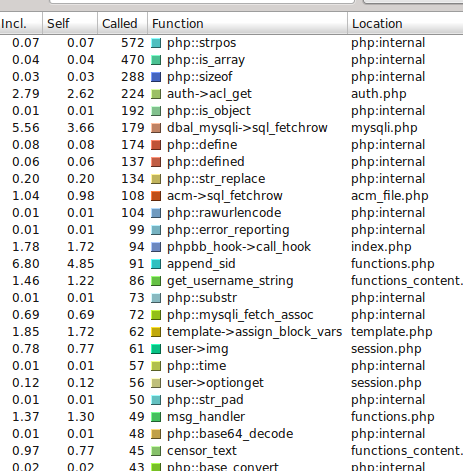
\includegraphics[scale=0.69]{rId45.png}
  \end{center}
  \vspace{0pt}
	\caption{Functions usage in KCacheGrind\label{rId45.png}}
  %\vspace{-10pt}
\end{wrapfigure}
\end{comment}
We see a different view this time, \textbf{common.php} (\autoref{rId45.png} on page~\pageref{rId45.png}) is using only 28\% of the time, the rest is for other things. Now let's see what functions are being used the most, and the time it takes for them to run. Maybe we can optimise something there. We can conclude that for one simple page request the internal strpos() function is ran almost 572 times. Since it's an internal function, and it doesn't use too many time it will be neglected, the same for the rest of the internals.
\img[h!]{scale=0.7}{rId45.png}{Functions usage in KCacheGrind}

\subsection{Conclusion}
Optimisation is not only about coding but also about avoiding bottlenecks. They can be numerous including network latency, processor load, file system speed.
Threading and processes creation, memory leaks, depending on external services is very slow if you require a lot of data.

There are a few techniques for databases, using caching instead of regenerating the same content. 
Remember to always reprofile your software using Valgrind or Xdebug.

Moving your \gls{apache} files and \gls{mysql} databases to a \gls{ssd} (or more if you want SSD RAID) helps avoinding disk latency.

\section{vApus test cases for phpBB}\label{sec:testcasesphpBB}
\gls{vapus} stands for Virtualized Application Unique Stresstesting and it can be used to stresstest anything. It works in a master-client way that can be used to stresstest different types of applications including databases, php websites or any other program. It also can be used to test a full server to its full potential.

vApus should be run as a test client on another pc than your development one, I'm using a quadcore client on the ip of 192.168.35.145. It's currently being controlled by RDP.

First import the \underline{Log Rule} set \textbf{Web Log Rule Set.xml}. Then import the Log 1: HTTP stresstest from the vApus mark II. Import a connection proxy: \textbf{Web HTTP (GZip Encoding, ignore logged cookies) Connection Proxy.xml}. Create a new connection with the website used. Add a new stresstest and configure it to use the logs imported.
\\But you can also use the pre-set settings and only use stresstest.

We have two stresstests. An original one using the path to /phpbb/ and a phpBB optimised using a path to /phpbboptimized/. The original one is started only once and then we compare it to the changes done with the optimised one.

Run the \textbf{importmysqldb.sh} script I made based on the info from the wiki so the \gls{mysql} database is reset after every usage. This script should reset both databases for the /phpbb/ and /phpbboptimized/ subdirectories. 

\subsection{Tools used and setup}
\subsubsection{Configuration and files}
This is our system setup and all the data locations, configuration files, versions of the software we'll use.

\begin{table}[htb!]\begin{center}
\caption{Table containing all the information of the different softwares used}\label{tab:configuration}
\arrayrulecolor{myLightGreen}
\begin{tabular}{|p{3cm}|p{3cm}|c|}\hline %\rowcolor{myLightGreen}
% & \multicolumn{2}{>{\columncolor{myLightGreen}}c|}{\bf\color{white} After APC} & \multicolumn{2}{>{\columncolor{myLightGreen}}c|}{\bf\color{white} Before APC} \\ \hline  \rowcolor{myLightGreen}
 %{\bf\color{white} Concurrent Users} & {\bf\color{white} Throughput / s} & {\bf\color{white} Response Time in ms} & {\bf\color{white} Throughput / s} & {\bf\color{white} Response Time in ms}  \\ \hline 
 
Operating system &	\multicolumn{2}{>{}c|}{\textbf{Ubuntu 11.10 64bit}} \\ \hline
CPU &  \multicolumn{2}{>{}c|}{2x Intel(R) Xeon(R) CPU  L5520  @ 2.27GHz, 4 cores, 8 threads} \\ \hline
RAM & 8GB & APC version 3.1.10  \\ \hline \rowcolor{myLightGreen}
%\multicolumn{3}{>{\columncolor{myLightGreen}}c|}{\bf\color{white} Software info}  \\ \hline
\rowcolor{myLightGreen} {\bf\color{white} Version}	& {\bf\color{white} Files} & {\bf\color{white} Configuration} \\ \hline{}
Apache  2.2.20 &  /mnt/raid/www  &  /etc/apache2/apache2.conf \\ \hline
MySQL  5.5.24.1 &  /mnt/raid/mysql &  /etc/mysql/my.cnf \\ \hline
PHP   5.4.0 & /mnt/raid/www & /etc/php5/apache2/php.ini \\ \hline 
% 200 & 1403.0 & 51.5 & 1327.6 & 58.7 \\ \hline \rowcolor{rowhighlight}

\end{tabular}\end{center}
\end{table}
\subsubsection{Using dstat and top when stresstesting with vApus}
First of all \gls{vapus} uses a \textbf{dstat} monitoring agent for the information we need. \textbf{Dstat} can be configured to give us detailed information. One big good thing about the intern dstat monitoring is that it automatically generates CSV/TSV's that can be imported in Excel or any other program to generate graphics. 

My main problem now is that I require something to view which applications use most of the memory so I'll have to import TOP data and also Input Output statistics from each device SSD/HDD to view if there are bottlenecks. That data isn't CSV friendly so I need to import it in another manner.

The stresstests we'll do requires that we know what processes are using most of the memory, \gls{cpu}, IO so we filter them and see what we can optimise. Top remains the best app for such things.

Starting \gls{vapus} and at the same moment issuing the top command to read everything:
\begin{codelisting}
top -b > topOutput.txt
\end{codelisting}
The data that we get from the dstat agent, \gls{vapus} monitoring stresstest and \textbf{top} is a lot to edit every time in Excel so a little automatization project has been started; first I needed to inspect what I will actually use. The idea is to save the data in a Sqlite database,  plot the data as you wish, export them to images 
and also maybe export everything to a \gls{html} file so it could be accessible for everyone. This will be explained in (add section reference here) \gls{tcl} script to plot charts.

Please note that some tests will be redone because this is research and in research we need to retest the same thing over and over and also to refine our tests. Trial and error is our friend as in every other research on earth. Some tests were not included because they were missing information or had been incorrect, some failed tests are explained to give us a better understanding of what went wrong and how we fixed some things. 
For a list of all the test files refer to the Appendix.

\subsubsection{First test case}
The first test case was a simple one using all 16 cores with a concurrency of 5, 100 and 250 clients.

We saw that the \gls{cpu} usage wasn't so high, it peaks at a total of 30 sometimes since there are 16 cores, maybe disabling 8 cores and testing again could result something else? A maximum of 2000 mb of memory were used at the start of the 250 concurrent clients. Writes up to 1.2 MB/sec have been noted
The latency is a little bad sometimes after viewing some other files.

Now I still have to see which process uses the most information so a little script to filter that out is also helpful. More details about this in \autoref{sec:scripts}.
\subsubsection{Failed test case with 8 cores}
After discussing with my coach and someone else from the team, a few problems have been spotted. The first problem is that there were some 403 FORBIDDEN errors, the LOGIN command in vApus wasn't pinned down as the first so I have to redo the tests.

The second problem was that \gls{hyperthreading} might be enabled; I had to disable it and then test everything again with 1, 2, 4 and 8 cores to \textbf{\underline{see if it scales}}. Because \gls{hyperthreading} isn't really a full scale core and it can improve the actual speed anywhere from 10\% to 50% so the test output can't be too reliable while we want to view the scaling. In production environments or when we'll start to optimise, this is important but now we'll disable it. This setting can easily be changed in BIOS.

Because we're using Linux we can change the system in almost any way we want without having to install too many programs or to dig into the internals like we'd do in Windows. It's fairly easy to disable some cores and enable them \textbf{\underline{while}} the system is running.

The following code disables the last 7 cores one by one and then gets the information to see if they really are disabled. To re-enable the cores change the 0 to 1 at the echo. Please do note that the core count starts from 0.
\begin{codelisting}
sudo bash
for i in {1..7};  do
	echo "Disabling CPU$i"
	echo 0 > /sys/devices/system/cpu/cpu$i/online
done
grep "processor" /proc/cpuinfo
\end{codelisting}

Before we start the stresstest, we have to reset the database like shown in a previous chapter.

It would have been great if we had been able to use \textbf{top} and iostat or \textbf{sar} within \textbf{dstat} so I wouldn't have to log everything separate. So maybe there are options in dstat self already knowing that it contains many default plugin's.

List all the \textbf{dstat} internal functions but also plug-in's.
\begin{codelisting}
lostone@chenbro-nehalem:~$ dstat --list
internal:
	aio, cpu, cpu24, disk, disk24, disk24old, epoch, fs, int, int24, io, ipc, 	load, lock, mem, net, page, page24, proc, raw, socket, swap, swapold, sys, 	tcp, time, udp, unix, vm
/usr/share/dstat:
	battery, battery-remain, cpufreq, dbus, disk-tps, disk-util, dstat, dstat-cpu, dstat-ctxt, dstat-mem, fan, freespace, gpfs, gpfs-ops, helloworld, innodb-buffer, innodb-io, innodb-ops, lustre, memcache-hits, mysql-io, 	mysql-keys, mysql5-cmds, mysql5-io, mysql5-keys, net-packets, nfs3, nfs3-ops, nfsd3, nfsd3-ops, ntp, postfix, power, proc-count, qmail, rpc, rpcd, sendmail, snooze, squid, test, thermal, top-bio, top-bio-adv, top-childwait, top-cpu, top-cpu-adv, top-cputime, top-cputime-avg, top-int, top-io, top-io-adv, top-latency, top-latency-avg, top-mem, top-oom, utmp, vm-memctl, vmk-hba, vmk-int, vmk-nic, vz-cpu, vz-io, vz-ubc, wifi
\end{codelisting}%$
Too bad that none of them actually do what we need so I guess it will have to be done manually using top and sar.

Instead of opening two terminals we can run both tests in one command:
\begin{codelisting}
sar -p -d 1 > 16cores_test_sar.txt & top -b > 16cores_test_top.txt 
\end{codelisting}
To stop it just press CTRL+C, and don't forget to \textbf{pkill} sar since it will still actively write to the file.

The value that interests us the most from \textbf{sar} is \textbf{avgqu-sz}. This is the average queue length of the requests that were issued to the device and if it's above 1 for a longer time then there is a bottleneck for the disk IO.

The \textbf{top} command produces a lot of output so filtering it is a job for a script.
\subsection{Simple scaling example}
\subsubsection{Test case with 1 core}
In a normal production environment we'd only get CPU and memory usage information for the server itself but since we need more information we'll have to log different things every second so this logging will have an effect on the CPU usage and some disk IO for the SATA disk. This isn't that bad since we'll be using the same test patterns for every disk and thus everything will be uniform. Even the growth with the cores should be constant and uniform.
\begin{codelisting}
sudo bash
for i in {1..7};  do
	echo "Disabling CPU$i"
	echo 0 > /sys/devices/system/cpu/cpu$i/online
done
grep "processor" /proc/cpuinfo
\end{codelisting}
Reset the \gls{mysql} database:
\begin{codelisting}
cd scripts
./importmysqldb.sh
\end{codelisting}
Start the IO logger and top. We're using SAR instead of iostats because of the better structure we get.
\begin{codelisting}
sar -p -d 1 > stresstest_1core_iosar.txt & top -b > stresstest_1core_procs.txt
\end{codelisting}

First I have started vApus with 25, 100 and 200 concurrent users. There were some errors again. After spending a few hours searching and then talking to one of my colleagues Liz, we finally made some changes to the vApus file and fixed everything, now it works. I wasn't using variables, so I always got redirects and because of that it took the tests way longer than normal. This test has been redone with 25,50,100,150,200 concurrent users.  Because this is our first test we'll show all the graphics, but for the next tests we'll only show the graphics that have changed or things that differ. 

Looking at \autoref{tab:1core} we can see that the maximum throughput is somewhere between 25 and 50 concurrent users so we'll need to redo this test later for more accurate information.
\begin{table}[ht!]
\begin{center}
\caption{Throughput and response time for 1 core}
\label{tab:1core}
\begin{tabular}[ht!]{|p{2.2cm}|p{2.2cm}|p{2.2cm}|}\hline\rowcolor{myLightGreen}\arrayrulecolor{myLightGreen}
 {\bf\color{white} Concurrent Users} & {\bf\color{white} Throughput / s} & {\bf\color{white} Response Time in ms} \\ \hline 
 25 & 160.5 & 63.9 \\ \hline  \rowcolor{rowhighlight} 
 50 & 161.5 & 216.6 \\ \hline 
 100 & 146.7 & 589.5 \\ \hline 
 150 & 141.5 & 963.3 \\ \hline 
 200 & 144.2 & 1298.2 \\ \hline 
\end{tabular}
\end{center}
\end{table}
What we can conclude is that there is a very high CPU usage when looking at \autoref{rId47.png}. 
\\The memory grows steadily but doesn't surpass 2500 MB (\autoref{rId48.png} on page \pageref{rId48.png}).
\\The disk usage has a few peaks but is still underused (\autoref{rId49.png} on page \pageref{rId49.png}). 
\\The network transfer is very low one peak of 5.1 MBps and the average is around 800KBps (\autoref{rId51.png} on page \pageref{rId51.png}).
\\The average queue isn't that bad either (\autoref{rId50.png} on page \pageref{rId50.png}).

\img[h!]{scale=0.5}{rId47.png}{CPU usage 1 core test}
\img[h!]{scale=0.5}{rId48.png}{Memory usage 1 core test} 
\img[h!]{scale=0.5}{rId49.png}{Disk usage 1 core test}
\img[h!]{scale=0.5}{rId50.png}{Average queue size 1 core test}
\img[h!]{scale=0.5}{rId51.png}{Network traffic 1 core test}
\clearpage{}%Leaves all the images BEFORE the next subsection, otherwise they'd tend to go to the end of the document

\subsubsection{Test case with 2 cores}
Enable core 2:
\begin{codelisting}
sudo bash
echo 1 > /sys/devices/system/cpu/cpu1/online
\end{codelisting}
The rest of the steps are the same, reset the DB, start the logging and start \gls{vapus} stresstesting.

The funny thing about this test was that I had Fiddler (a proxy) open on the client machine that ran vApus and it began using 3 GB of memory thus the testing wasn't what it should have been so I had to redo the tests so that the logs would be accurate.

\begin{table}[ht!]
\begin{center}
\caption{Throughput and response time for 2 core} \label{tab:2cores}
\begin{tabular}{|p{2.2cm}|p{2.2cm}|p{2.2cm}|}\hline\rowcolor{myLightGreen}\arrayrulecolor{myLightGreen}
 {\bf\color{white} Concurrent Users} & {\bf\color{white} Throughput / s} & {\bf\color{white} Response Time in ms} \\ \hline 
 25 & 199.8 & 29.9 \\ \hline 
 50 & 338.7 & 52.5 \\ \hline \rowcolor{rowhighlight}
 100 & 362.4 & 183.1 \\ \hline 
 150 & 335.7 & 353.8 \\ \hline 
 200 & 311.8 & 548.8 \\ \hline 
\end{tabular}
\end{center}
\end{table}
The throughput and response time is at its highest for 100 concurrent users (\autoref{tab:2cores}).

CPU usage is as high as before (\autoref{rId52.png} on page \pageref{rId52.png}).

The memory seems to be the same  (\autoref{rId53.png} on page \pageref{rId53.png}).

The disk usage is a little lower than before, with just 2 peaks above 2 MB. There are fewer peaks above one MB than with 1 core (\autoref{rId54.png} on page \pageref{rId54.png}).

The network traffic has grown a little bit  (\autoref{rId56.png} on page \pageref{rId56.png}).
\img[h!]{scale=0.5}{rId52.png}{CPU usage 2 cores test}
\img[h!]{scale=0.5}{rId53.png}{Memory usage 2 cores test}
\img[h!]{scale=0.5}{rId54.png}{Disk usage 2 cores test}
%add the disk queue here? \img[h!]{scale=0.5}{rId55.png}{Average queue size 2 cores test}
\img[h!]{scale=0.5}{rId56.png}{Network traffic 2 cores test}
\clearpage{}

\subsubsection{Test case with 4 cores}
Everything that you have to set up is the same as the other settings except that you have to enable another 2 cores. For this test we'll add 300 extra concurrent users at the end.
\begin{codelisting}
sudo bash
echo 1 > /sys/devices/system/cpu/cpu2/online
echo 1 > /sys/devices/system/cpu/cpu3/online
\end{codelisting}
Again as in the past examples reset the database, start the TOP and SAR log's and start \gls{vapus}.
The best results are for 200 concurrent users. The throughput tripled and the concurrent users doubled with a lower time than before (\autoref{tab:4cores}).
\begin{table}[ht!]\begin{center}
\caption{Throughput and response time for 4 cores}\label{tab:4cores}
\begin{tabular}{|p{2.2cm}|p{2.2cm}|p{2.2cm}|}\hline\rowcolor{myLightGreen}\arrayrulecolor{myLightGreen}
 {\bf\color{white} Concurrent Users} & {\bf\color{white} Throughput / s} & {\bf\color{white} Response Time in ms} \\ \hline 
 25 & 217.4 & 21.9 \\ \hline 
 50 & 386.6 & 34.9 \\ \hline 
 100 & 704.5 & 49.2 \\ \hline 
 150 & 901.9 & 73.1 \\ \hline \rowcolor{rowhighlight}
 200 & 942.8 & 119.5 \\ \hline 
 300 & 753.9 & 308.4 \\ \hline 
\end{tabular}\end{center}
\end{table}

The CPU usage seems lower at the beginning, and it's higher only for a short period of time, 200 samples instead of 150 for the 1 core version (\autoref{rId57.png} on page \pageref{rId57.png}).

The peak memory is only for a short while and it decreases to around 1190 MB. It's stable and it doesn't persist too much (\autoref{rId58.png} on page \pageref{rId58.png}).

We can clearly see network peaks that are larger than in the example with 1 or 2 cores. But this is because it must send more data in less time. It still scales with no problem (\autoref{rId61.png} on page \pageref{rId61.png}).
\img[h!]{scale=0.37}{rId61.png}{Network traffic 4 cores test}
\img[h!]{scale=0.5}{rId57.png}{CPU usage 4 cores test}
\img[h!]{scale=0.5}{rId58.png}{Memory usage 4 cores test}
%disk IO & disk queue neglected..?

\clearpage{}

\subsubsection{Test case with 8 cores}
Everything that you have to set up is the same as the other settings except that you have to enable another 8 cores. Another 400 concurrent users where added to vApus.
\begin{codelisting}
sudo bash
for i in {4..7};  do
	echo "Enabling CPU$i"
	echo 1 > /sys/devices/system/cpu/cpu$i/online
done
grep "processor" /proc/cpuinfo
\end{codelisting}
The throughput doubled again but this time only 300 concurrent users where served and it seems that the response time is stable (\autoref{tab:8cores}).
\begin{table}[ht!]
\begin{center}
\caption{Throughput and response time for 8 cores}\label{tab:8cores}
\begin{tabular}{|p{2.2cm}|p{2.2cm}|p{2.2cm}|}\hline\rowcolor{myLightGreen}\arrayrulecolor{myLightGreen}
 {\bf\color{white} Concurrent Users} & {\bf\color{white} Throughput / s} & {\bf\color{white} Response Time in ms} \\ \hline 
 25 & 214.7 & 24.5 \\ \hline 
 50 & 391.8 & 33.7 \\ \hline 
 100 & 740.7 & 41.8 \\ \hline 
 150 & 1034.0 & 52.4 \\ \hline 
 200 & 1331.8 & 58.1 \\ \hline \rowcolor{rowhighlight}
 300 & 1624.8 & 93.4 \\ \hline 
 400 & 1560.4 & 168.4 \\ \hline 
\end{tabular}\end{center}
\end{table}

The CPU usage is very stable with only momentary high peaks. The higher CPU time for 400 concurrent users is normal since we see that the request time is lower because of too many requests. (\autoref{rId62.png} on page \pageref{rId62.png}).

The memory scales very well, nothing new here, the maximum values are taking less time and they're decreasing to a lower value (\autoref{rId63.png} on page \pageref{rId63.png}).

%disk usage not included..? negligible
Again, the network traffic grows with the total number of concurrent users but it all gets sent so nothing is left behind (\autoref{rId65.png} on page \pageref{rId65.png}). It scales well
\img[h!]{scale=0.5}{rId62.png}{CPU usage 8 cores test}
\img[h!]{scale=0.5}{rId63.png}{Memory usage 8 cores test}
\img[h!]{scale=0.5}{rId65.png}{Network traffic 8 cores test}
\clearpage{}
\subsubsection{1 Core with more steps and warming up for a better overview}
\begin{wraptable}{r}{0.5\columnwidth}
\begin{centering}
\caption{Throughput and response time for 1 core with more steps}\label{tab:1coremoresteps}
\begin{tabular}{|p{2.2cm}|p{2.3cm}|p{2.3cm}|}\hline\rowcolor{myLightGreen}\arrayrulecolor{myLightGreen}
 {\bf\color{white} Concurrent Users} & {\bf\color{white} Throughput / s} & {\bf\color{white} Response Time in ms} \\ \hline 
 5 & 44.2 & 18.6 \\ \hline 
 15 & 112.9 & 33.7 \\ \hline \rowcolor{rowhighlight} 
 25 & 157.1 & 62.9 \\ \hline \rowcolor{rowhighlight}
 35 & 177.1 & 103.0 \\ \hline 
 50 & 167.0 & 204.8 \\ \hline 
 75 & 153.3 & 396.3 \\ \hline 
 100 & 152.0 & 563.6 \\ \hline 
 115 & 148.1 & 683.1 \\ \hline 
 130 & 134.4 & 998.1 \\ \hline 
\end{tabular}
\end{centering}
\end{wraptable}
A better way to view where 1 core scales the best is to add more steps. Also added 5 and 15 steps for the time it requires to start the Apache processes.  We have used the following number of concurrent users: 5,15,25,35,50,75,100,115,130,150,175

The test was stopped when it passed 130 concurrent users because have already reached the highest throughput anyway.
What is interesting now is to see the fast results from vApus.
We see (\autoref{tab:1coremoresteps}) that the maximum thorughput is 177 requests per second and the response time is 102 ms at 35 concurrent users. After this the response time doubles and the throughput gets lower. For 1 core we'll conclude that phpBB and Apache meet their maximum at 35 concurrent users.
For one core we'll conclude that the highest thorughput and best responsetime is for 35 concurrent users.

\subsubsection{Conclusions for 1 to 8 cores tests}
As the core count grows everything scales with it(\autoref{tab:1to8cores}). The network traffic is higher with each new core but this is normal and logical because it sends more data in less time. The tests complete faster so there are fewer steps in between. 

\begin{table}[ht!]\begin{center}
\caption{Throughput and Response Time for 1 to 8 cores}\label{tab:1to8cores}
\begin{tabular}{|p{1.5cm}|p{1.4cm}|p{1.4cm}|p{1.4cm}|p{1.4cm}|p{1.4cm}|p{1.4cm}|p{1.4cm}|p{1.4cm}|}\hline\rowcolor{myLightGreen}\arrayrulecolor{myLightGreen}
  &  \multicolumn{2}{>{\columncolor{myLightGreen}}c|}{\bf\color{white} 1 core} & \multicolumn{2}{>{\columncolor{myLightGreen}}c|}{\bf\color{white} 2 cores} & \multicolumn{2}{>{\columncolor{myLightGreen}}c|}{\bf\color{white} 4 cores} & \multicolumn{2}{>{\columncolor{myLightGreen}}c|}{\bf\color{white} 8 cores} \\ \hline  \rowcolor{myLightGreen}
 {\bf\color{white} Concurrent Users} & {\bf\color{white} Thr / s} & {\bf\color{white} Resp Time / ms} & {\bf\color{white} Thr / s} & {\bf\color{white} Resp Time / ms} & {\bf\color{white} Thr/ s} & {\bf\color{white} Resp Time / ms} & {\bf\color{white} Thr / s} & {\bf\color{white} Resp Time / ms} \\ \hline 
 25 & 160.5 & 63.9 & 199.8 & 29.9  & 217.4 & 21.9 & 214.7 & 24.5 \\ \hline
 50 & \bf 161.5 &  \bf 216.6 & \bf 338.7 & \bf 52.5 &  386.6 & 34.9 & 391.8 & 33.8 \\ \hline
 100 & 146.7 & 589.5 & \bf 362.4 & \bf 183.1 &  704.5 & 49.2 & 740.7 & 41.8 \\ \hline
 150 & 141.5 & 963.3 & 335.7 & 353.8 &  901.9 & 73.2 & 1034.0 & 52.4 \\ \hline
 200 & 144.2 & 1298.2 & 311.8 & 548.8 & \bf  942.8 & \bf 119.5 & 1331.8 & 58.1 \\ \hline
 300 &  &  &  &  &  753.9 & 308.4 & \bf 1624.8 & \bf 93.5 \\ \hline
 400 &  &  &  &  &   &  & 1560.4 & 168.4 \\ \hline
\end{tabular}\end{center}
\end{table}
For 2 cores the throughput doubles and the response time is halved for the same amount of users(50). For 4 cores the concurrent users have a tripled throughput with a relative good response time of 120 ms.
\img[h!]{}{throughput1to8cores.png}{Throughput per second for 1 to 8 cores}
From both graphics (\autoref{throughput1to8cores.png} on page \pageref{throughput1to8cores.png}) and (\autoref{responsetime1to8cores.png} on page \pageref{responsetime1to8cores.png}) we can conclude that as the core count doubles so does the maximum throughput for the stress tests. 
\img[h!]{}{responsetime1to8cores.png}{Response Time in ms for 1 to 8 cores}
Once the optimal number of concurrent users has been reached for any stress test the response time is almost exponential (\autoref{responsetime1to8cores.png} on page \pageref{responsetime1to8cores.png}). The 1 core actually hits 1300 but it has been capped at 500 so we see the rest clearly.

\clearpage{}
\subsection{Tweaking the Apache settings}
Being sure that \gls{apache} uses the \textbf{gzip} and mod\_deflate to send compressed data to the browser and to \gls{vapus} so we decrease the total network traffic, this is a form of optimisation. It should be on by default in the newer versions, but it's provided as a help.

Changes in \textbf{/etc/apache2/apache2.conf}
\begin{codelisting}
SetOutputFilter DEFLATE
BrowserMatch ^Mozilla/4\.0[678] no-gzip\
BrowserMatch \bMSI[E] !no-gzip !gzip-only-text/html
# Don't compress images
SetEnvIfNoCase Request_URI \\.(?:gif|jpe?g|png)\$ no-gzip dont-vary
\end{codelisting}
Edit the \textbf{/etc/apache/mods/mod\_deflate.conf }file.
\begin{codelisting}
AddOutputFilterByType DEFLATE text/html text/plain text/xml text/css application/x-javascript application/javascript application/ecmascript application/rss+xml text/x-js
BrowserMatch ^Mozilla/4 gzip-only-text/html
BrowserMatch ^Mozilla/4\.0[678] no-gzip
BrowserMatch \bMSIE !no-gzip !gzip-only-text/html
\end{codelisting}
Because of the information provided by \textbf{YSlow} and \textbf{Google's PageSpeed} (\autoref{subsec:frontend}) applications we have concluded that we need to add caching to all our files. This is best done in \gls{apache}. Caching of files to the client helps us have a lower page load time if we use the site a longer time. It decreases traffic for the server so it's good. Caching stuff, this is best so the users won't request them anymore. This is one optimisation we won't be able to test because we are not using a browser to stresstest it and \gls{vapus} always gets all the files, it doesn't cache anything. 

Install the \gls{apache} \textbf{expires} module.\cite{optimizing_LAMP_helioviewer}
\begin{codelisting}
sudo a2enmod expires
\end{codelisting}
Next, edit \textbf{/etc/apache2/mods-enabled/expires.conf} and add the following section:
\begin{codelisting}
<IfModule mod_expires.c>
      ExpiresActive On
      ExpiresByType image/x-icon "access plus 1 year"
      ExpiresByType image/png "access plus 3 months"
      ExpiresByType image/jpg "access plus 3 months"
      ExpiresByType image/gif "access plus 3 months"
      ExpiresByType image/jpeg "access plus 3 months"
      ExpiresByType video/ogg "access plus 1 month"
      ExpiresByType video/mpeg "access plus 1 month"
      ExpiresByType video/mp4 "access plus 1 month"
      ExpiresByType video/quicktime "access plus 1 month"
      ExpiresByType video/x-ms-wmv "access plus 1 month"
      ExpiresByType text/css "access plus 3 months"
      ExpiresByType text/html "access plus 3 months"
      ExpiresByType text/javascript "access plus 3 months"
      ExpiresByType application/javascript "access plus 3 months"
</IfModule>
\end{codelisting}
After doing this the pagespeed score 99/100 and it used to be 80! The YSlow is also 99 and it was 77.
\clearpage{}
\subsection{Update phpBB 3.0.5 to 3.0.10}
We'll update the phpBB forum installation to see if it runs faster. We also want to be able to use \gls{memcached} later to see if there is any speed difference. Although \gls{memcached} is made for distributed computing we should be able to view a change because it saves everything in memory instead of reading from the disk.

Extract the contents of the update archive to \textbf{/mnt/raid/www/phpbboptimized/}.
First we change the name of the \textbf{degrensstreek} database in the \textbf{degrensstreek2.sql} file that we save, we change our script to import both databases at the same time.
Then we edit \textbf{config.php}
\begin{codelisting}
$dbname = 'degrensstreek2';
\end{codelisting}%$
Run the ./importmysqldb.sh to change the database. Following: http://yoursite/install/index.php

This updates the database, it collects the FILE differences of each file and prompts with more information about each file then you can either use FTP to update them or just download.  Now a fun part, if you want to download the files you get a tar.gz from the host where you tried to update it to manually copy the files. I find this stupid because phpBB can copy them directly using \gls{php}!

Change the location of the folder's place in \gls{vapus}.
Problems: when I ran the script to reset the database, it actually reset everything to the old version that wouldn't work. So I had to redo the installation and backup the database first!

Don't forget to edit the \gls{vapus} HTTP log at the \textbf{ViewTopic} link, it must become  \textbf{/phpbboptimized/viewtopic.php} instead of \textbf{/phpbboptimized/viewforum.php}.

Also update the degrensstreek2.sql and add the following code at the top:
\begin{codelisting}
CREATE DATABASE /*!32312 IF NOT EXISTS*/ `degrensstreek2` /*!40100 DEFAULT CHARACTER SET latin1 */;
USE `degrensstreek2`;
\end{codelisting}
The graphics are almost all the same as previous tests, it scales great. The optimized phpBB with 8 cores uses 300 more MB than the previous version, the scaling is the same. It could be that there is some other process running in the \gls{ram}.
What is interesting now is to see the fast results from \gls{vapus} in \autoref{tab:phpbbUpgrade}.

Just as the normal 8 cores test, at 300 concurrent users we see a throughput of 1611 requests per second and a average response time of 95 ms. This is the maximum, for more concurrent users it just gets worse.

\begin{table}[htb!]\begin{center}
\caption{Differencing response time and throughput after phpBB upgrade}\label{tab:phpbbUpgrade}
\begin{tabular}{|p{2.3cm}|p{2.3cm}|p{2.3cm}|p{2.3cm}|p{2.3cm}|}\hline\rowcolor{myLightGreen}\arrayrulecolor{myLightGreen}
 & \multicolumn{2}{>{\columncolor{myLightGreen}}c|}{\bf\color{white} Before upgrade} & \multicolumn{2}{>{\columncolor{myLightGreen}}c|}{\bf\color{white} After upgrade} \\ \hline  \rowcolor{myLightGreen}
 {\bf\color{white} Concurrent Users} & {\bf\color{white} Throughput / s} &  {\bf\color{white} Response Time in ms} & {\bf\color{white} Throughput / s} & {\bf\color{white} Response Time in ms} \\ \hline 
 100 & 740.7 & 41.8 & 753.1 & 41.3 \\ \hline 
 150 & 1034.0 &  52.4 & 1039.8 & 52.2 \\ \hline 
 200 & 1331.8 &  58.1 & 1330.8 & 59.1 \\ \hline 
 300 & 1624.8 & 93.4 & 1611.9 & 95.3 \\ \hline 
 400 & 1560.4 & 168.4 & 1558.9 & 167.4 \\ \hline 
\end{tabular}\end{center}
\end{table}
%PHPBB cache changes for 8 cores
\clearpage
\subsection{phpBB cache changes for 8 cores}
\subsubsection{No cache enabled}
This is a test done with no cache enabled. To disable caching in phpBB just edit the config.php file:
\begin{codelisting}
$acm_type = 'null';
\end{codelisting}%$
We see that the maximum throughput is 1521 requests per second and that the response time is 106. Our conclusion for this test is that caching in phpBB is efficient! 
\subsubsection{Memcached enabled}
\gls{memcached} is a server application that stores data for other applications in memory so it can work faster, it caches things it needs. It's very useful for caching static data or existing forum posts that haven't been altered in some time.
To enable memcache just edit the config.php file:
\begin{codelisting}
$acm_type = 'memcache';
\end{codelisting}%$
The maximum throughput for this test is 1528 and a response time of 105, this caches everything in memory but still we see no difference. Let's look at some graphics this time, not everything seems the same.

The CPU seems to be the same as the file cache. 

The disk queue is stable and the network traffic seems to scale the same way.

The disk usage has a lot of peaks and goes a lot above 10 MBps. This wasn't so for the normal 8 core test not even for the updated version of phpBB (\autoref{rId69.png} on page \pageref{rId69.png}).

The memory usage is \textbf{doubled} if you want to compare to the normal 8 cores test which uses 2.7 GB RAM and now the maximum peak is 5.2 GB (\autoref{rId70.png} on page \pageref{rId70.png}).

A simple conclusion is that enabling \gls{memcached} actually uses more memory, and it writes even more to the hard disk, it's not known why. File cache seems faster.
\img[htb!]{scale=0.5}{rId69.png}{Disk usage for 8 cores test with memcached enables}
\img[htb!]{scale=0.5}{rId70.png}{Memory usage for 8 cores test with memcached enables}
\clearpage{}
\subsubsection{Conclusion for 8 cores with no cache and Memcached tests}
Looking at \autoref{tab:8coresmemcached} we can conclude that there is no real difference between the \gls{memcached} settings and if no cache at all would be enabled (meaning everything would be regenerated at every request). This means that memcached doesn't have any speed impact on a webserver unless it's used from multiple servers.

\begin{table}[htb!]\begin{center}
\caption{Throughput and Response time for 8 cores comparing no cache settings with Memcached}\label{tab:8coresmemcached}
\begin{tabular}{|p{2.2cm}|p{2.2cm}|p{2.2cm}|p{2.2cm}|p{2.2cm}|}\hline\rowcolor{myLightGreen}\arrayrulecolor{myLightGreen} 
& \multicolumn{2}{>{\columncolor{myLightGreen}}c|}{\bf\color{white} No cache} & \multicolumn{2}{>{\columncolor{myLightGreen}}c|}{\bf\color{white} Memcached} \\ \hline \rowcolor{myLightGreen}
 {\bf\color{white} Concurrent Users} & {\bf\color{white} Throughput / s} & {\bf\color{white} Response Time in ms} & {\bf\color{white} Throughput / s} & {\bf\color{white} Response Time in ms} \\ \hline 
 25 & 210.8 & 24.3 & 206.0 & 28.0 \\ \hline 
 50 & 394.0 &  33.3 & 387.6 & 32.5 \\ \hline 
 100 & 741.4 &  41.6 & 741.7 & 41.8 \\ \hline 
 150 & 1017.7 & 54.4 & 1017.8 & 55.5 \\ \hline 
 200 & 1285.8 &  63.9 & 1269.2 & 66.6 \\ \hline 
 300 & 1521.5 &  106.7 & 1528.3 & 105.4 \\ \hline 
 400 & 1431.8 &  200.6 & 1450.7 & 192.4 \\ \hline 
\end{tabular}\end{center}
\end{table}

\subsection{Hyperthreading enabled to see how it scales}
Enabling \gls{hyperthreading} and doing an intensive test with more steps is required to be able to see what the real bottleneck would be in a production environment where we would use all the resources available.

From now on we'll have 16 cores (8 real cores with 2 threads each) with the following concurrent users to see where we'll find the maximum throughput: 5, 25, 50, 100, 200, 300, 325, 350, 375 and 400.

Here we'll do 2 tests, one with file cache where all the settings are the same as with the 8 cores and another with \gls{memcached} again. \gls{memcached} is just used to see how it scales on 16 cores. 
\subsubsection{16 cores with simple file cache}
It seems we can get up to 1753 requests per second at 375 concurrent users and an average response time of 126 ms. The \gls{hyperthreading} is doing its work. 
\subsubsection{16 cores with memcached on}
As we're used to this, the \gls{memcached} version uses almost double RAM. The disk write seems to be the same. IO sar doesn't report any disk problem so we're ok. 1733 maximum requests per second for 375 users with only a little higher average time of 129 ms.
\subsubsection{Conclusion for 16 cores test}
One interesting conclusion to note is that even if the throughput is lower for the \gls{memcached} test the response time is better than for the file cache starting from the 100 to the 375 concurrent users where it increases again. The memcached test at 300 concurrent users seems 25 ms faster with 105 more requests per second than the simple file cache.  
We'll notice that MySQL is using only 10\% of the total CPU.
\ref{tab:16coreCompare}
\begin{table}[ht!]\begin{center}
\caption{Throughput and Response time for 16 cores comparing simple file cache with memcached}\label{tab:16coreCompare}
\begin{tabular}{|p{2.2cm}|p{2.2cm}|p{2.2cm}|p{2.2cm}|p{2.2cm}|}\hline\rowcolor{myLightGreen}\arrayrulecolor{myLightGreen}
 & \multicolumn{2}{>{\columncolor{myLightGreen}}c|}{\bf\color{white} File cache} & \multicolumn{2}{>{\columncolor{myLightGreen}}c|}{\bf\color{white} Memcached} \\ \hline \rowcolor{myLightGreen}
 {\bf\color{white} Concurrent Users} & {\bf\color{white} Throughput / s} & {\bf\color{white} Response Time in ms} & {\bf\color{white} Throughput / s} & {\bf\color{white} Response Time in ms} \\ \hline 
 5 & 45.0 & 13.9 & 46.5 & 14.8 \\ \hline 
 25 & 212.3 &  26.8 & 204.3 & 27.4 \\ \hline 
 50 & 397.4 &  31.6 & 390.0 & 36.3 \\ \hline 
 100 & 702.2 &  49.4 & 719.0 & 46.4 \\ \hline 
 200 & 1290.4 &  63.2 & 1293.8 & 63.0 \\ \hline 
 300 & 1548.1 & 115.4 & 1653.4 & 90.9 \\ \hline 
 325 & 1581.4 &  128.0 & 1628.2 & 109.7 \\ \hline 
 350 & 1620.0 & 139.4 & 1685.8 & 121.3 \\ \hline 
 375 & 1753.3 &  126.8 & 1733.5 & 129.8 \\ \hline 
 400 & 1693.8 & 149.0 & 1644.2 & 161.9 \\ \hline 
\end{tabular}\end{center}
\end{table}

\img[htb!]{scale=0.3}{16_cores_cpu_intensive.png}{Apache and MySQL CPU usage}
\subsection{Changing Apache worker module settings}\label{subsec:changingApacheSettings}
One key to making Apache ,,work faster'' is to tweak the total number of start servers. Also play around with the maxClients, threads and MaxRequestsPerChild.
T
he MaxRequestsPerChild allows 2000 requests per child thread/server before it gets killed. This is useful because of possible memory leaks that could occur. 
\begin{codelisting}
<IfModule mpm_worker_module>
    StartServers          7
    MinSpareThreads      25
    MaxSpareThreads      75 
    ThreadLimit          64
    ThreadsPerChild      25
    MaxClients          300
    MaxRequestsPerChild   2000
</IfModule>
\end{codelisting}
\subsubsection{Worker module settings with simple file cache}
The examples in graphics aren't shown here because they scale the same way, however the memory does seem to go above 3 GB at some times (\autoref{rId71.png} on page \pageref{rId71.png}). Apache seems to use 32\% of the memory on an average in the total time of the test. That's a little more than when using less servers. 
We do get a higher throughput for a longer time than the previous tests. Looking at \autoref{newVSoldApache.png} on page \pageref{newVSoldApache.png} it seems that the new test is better.

\subsubsection{Differences between old and new Apache settings}

For the new \gls{apache} configuration we can observe that the throughput is higher and that the response time is lower. This test was a success between 100 and 375 concurrent users. From 400 upwards it begins to start losing its grip a little bit but that doesn't matter since the other differences are so big. (\autoref{tab:apacheNewAndOld})
\begin{table}[htb!]\begin{center}
\caption{Apache old vs new configuration differences}\label{tab:apacheNewAndOld}
\begin{tabular}{|p{2.2cm}|p{2.2cm}|p{2.2cm}|p{2.2cm}|p{2.2cm}|}\hline\rowcolor{myLightGreen}\arrayrulecolor{myLightGreen}
 & \multicolumn{2}{>{\columncolor{myLightGreen}}c|}{\bf\color{white} Old configuration} & \multicolumn{2}{>{\columncolor{myLightGreen}}c|}{\bf\color{white} New configuration} \\ \hline  \rowcolor{myLightGreen}
 {\bf\color{white} Concurrent Users} & {\bf\color{white} Throughput / s} & {\bf\color{white} Response Time in ms} & {\bf\color{white} Throughput / s} & {\bf\color{white} Response Time in ms} \\ \hline 
 5 & 45 & 13.9 & 46.6 & 16.9 \\ \hline 
 25 & 212.3 & 26.8 & 209 & 25 \\ \hline 
 50 & 397.4 & 31.6 & 393.2 & 34.2 \\ \hline 
 100 & 702.2 & 49.4 & 709.8 & 47.9 \\ \hline 
 200 & 1290.4 & 63.2 & 1327.6 & 58.7 \\ \hline 
 300 & 1548.1 & 115.4 & 1714 & 83.6 \\ \hline 
 325 & 1581.4 & 128 & 1734.5 & 96.1 \\ \hline 
 350 & 1620 & 139.4 & 1630.3 & 125.1 \\ \hline 
 375 & 1753.3 & 126.8 & 1746.1 & 126.2 \\ \hline 
 400 & 1693.8 & 149 & 1671.3 & 151.6 \\ \hline 
\end{tabular}\end{center}
\end{table}

\img[htb!]{}{newVSoldApache.png}{New vs old Apache configuration comparison}
\clearpage{}

\subsubsection{Comparing memcache tests with the new and old Apache settings}
All graphic have almost the same scaling as the previous \gls{memcached}. We're used to the poorer performance of \gls{memcached}.
You don't require a physics degree to see that the \gls{memcached} settings are bad in \autoref{tab:memcachedCompare}. If you recall the first 16 core memcached test, it's even worse than those (refresh your memory with \autoref{tab:16coreCompare} on page \pageref{tab:16coreCompare})
\begin{table}[htb!]\begin{center}
\caption{Comparing memcache tests with the new and old settings}\label{tab:memcachedCompare}
\begin{tabular}{|p{2.2cm}|p{2.2cm}|p{2.2cm}|p{2.2cm}|p{2.2cm}|}\hline\rowcolor{myLightGreen}\arrayrulecolor{myLightGreen}
& \multicolumn{2}{>{\columncolor{myLightGreen}}c|}{\bf\color{white} New settings} & \multicolumn{2}{>{\columncolor{myLightGreen}}c|}{\bf\color{white} Old settings} \\ \hline \rowcolor{myLightGreen}
 {\bf\color{white} Concurrent Users} & {\bf\color{white} Throughput / s} & {\bf\color{white} Response Time in ms} & {\bf\color{white} Throughput / s} & {\bf\color{white} Response Time in ms} \\ \hline 
 5 & 47.6 & 16.8 & 46.5 & 14.8 \\ \hline 
 25 & 214.2 &  24.2 & 204.3 & 27.4 \\ \hline 
 50 & 395.4 & 33.7 & 390.0 & 36.3 \\ \hline 
 100 & 737.0 & 43.6 & 719.0 & 46.4 \\ \hline 
 200 & 1254.1 & 66.2 & 1293.8 & 63.0 \\ \hline \rowcolor{rowhighlight}
 300 & 1648.7 & 93.5 & 1653.4 & 90.9 \\ \hline \rowcolor{rowhighlight}
 325 & 1661.5 & 104.6 & 1628.2 & 109.7 \\ \hline 
 350 & 1693.7 & 119.1 & 1685.8 & 121.3 \\ \hline \rowcolor{rowhighlight}
 375 & 1668.6 & 136.8 & 1733.5 & 129.8 \\ \hline 
 400 & 1600.6 & 163.0 & 1644.2 & 161.9 \\ \hline 
\end{tabular}\end{center}
\end{table}
\subsubsection{Conclusions for the new vs old Apache settings}
The new settings give the simple file cache a great boost between 100 and 375 users. It has a downside for the memcached one.
\subsection{Modifying memcache settings}
While searching the internet for tweakings and optimisations for memcached I found some info on how to change the total RAM that memcached can use.\cite{optimizing_memcached} I then saw that it had been using 64. I've changed that to 2048 MB of ram in the file /etc/memcached.conf. 
\\\textbf{-m 2048}

This was expected, it uses a little more average memory than the previous \gls{memcached} test but the peak isn't at the end of the test anymore but at the middle. As we can conclude from the vApus information and from the memory usage graphics:

The biggest peak is at 300 concurrent users, then at 325 where the memory already starts to be less (see \autoref{rId73.png} on page \pageref{rId73.png}). It's interesting to note that memory used for the 400 concurrent users is even lower than that of the simple file cache.
Probably running memcached in the long run on a webserver does have benefits of lesser cpu usage but it has way lower throughput and response time as to be seen in \autoref{tab:newmemcachedResults}.

\begin{table}[htb!]\begin{center}
\caption{Throughput results for new memcached settings}\label{tab:newmemcachedResults}
\begin{tabular}{|p{2.2cm}|p{2.3cm}|p{2.3cm}|}\hline\rowcolor{myLightGreen}\arrayrulecolor{myLightGreen}
 {\bf\color{white} Concurrent Users} & {\bf\color{white} Throughput / s} & {\bf\color{white} Response Time in ms} \\ \hline 
 5 & 47.6 & 18.2 \\ \hline 
 25 & 217.7 & 23.0 \\ \hline 
 50 & 393.8 & 34.4 \\ \hline 
 100 & 717.5 & 45.5 \\ \hline 
 200 & 1278.1 & 63.5 \\ \hline 
 300 & 1602.1 & 98.1 \\ \hline 
 325 & 1539.6 & 125.6 \\ \hline 
 350 & 1637.5 & 125.7 \\ \hline 
 375 & 1608.7 & 156.0 \\ \hline 
 400 & 1534.2 & 178.7 \\ \hline 
\end{tabular}\end{center}
\end{table}

%image here
\img[h!]{scale=0.5}{rId73.png}{Memcached new settings memory usage}
\clearpage{}

\subsection{Other Apache configuration settings}\label{subsec:apacheOtherSettings}
Changing the worker module settings again just to see how it scales.
\begin{codelisting}
<IfModule mpm_worker_module>
    StartServers          10
    MinSpareThreads      25
    MaxSpareThreads      75 
    ThreadLimit          64
    ThreadsPerChild      25
    MaxClients          300
    MaxRequestsPerChild   4000
</IfModule>
\end{codelisting}
I expected it to be better but it seems that the throughput and response time is far even from the unaltered settings of \gls{apache} in \autoref{tab:otherApache-settings}.

\begin{table}[ht!]\begin{center}
\caption{Other apache settings}\label{tab:otherApache-settings}
\begin{tabular}{|p{2.2cm}|p{2.3cm}|p{2.3cm}|}\hline\rowcolor{myLightGreen}\arrayrulecolor{myLightGreen}
 {\bf\color{white} Concurrent Users} & {\bf\color{white} Throughput / s} & {\bf\color{white} Response Time ms} \\ \hline 
 5 & 41.9 & 18.3 \\ \hline 
 25 & 209.4 & 25.1 \\ \hline 
 50 & 384.2 & 35.5 \\ \hline 
 100 & 728.9 & 44.0 \\ \hline 
 200 & 1289.3 & 63.0 \\ \hline 
 300 & 1522.8 & 117.6 \\ \hline 
 325 & 1609.2 & 121.5 \\ \hline 
 350 & 1437.7 & 163.6 \\ \hline 
 375 & 1592.0 & 167.8 \\ \hline 
 400 & 1511.9 & 184.4 \\ \hline 
\end{tabular}\end{center}
\end{table}
It uses more memory peaks that are above 4.3 GB of RAM and also the average is higher than the previous tests (see \autoref{rId74.png} on page \pageref{rId74.png}).

The disk write is also much higher than an usual test (see \autoref{rId75.png} on page \pageref{rId75.png}).

\img[h!]{scale=0.5}{rId74.png}{Other apache settings and memory usage}
\img[h!]{scale=0.5}{rId75.png}{High disk/write for the newest apache settings}
\clearpage{}
\subsection{New MySQL settings}
While searching the filesystem I noted that the place for the MySQL my.cnf settings was wrong, also the settings in that file where not correct since I've followed the CentOS directives and I'm using Ubuntu. The settings have to be changed and reimported. It's not expected that these settings would have too much of an impact on the end results so it will just be a new testcase.
As far as I've noted the only great difference is changing one file location with the other twice in my.cnf.
\begin{codelisting}
/var/lib/mysql/mysql.sock -> /var/run/mysqld/mysqld.sock
\end{codelisting}

Something bad must have happened because after the holiday it didn't work anymore.
Even after setting everything to the correct values, now MySQL won't connect anymore. Reinstalling everything was the only way to fix these problems otherwise nothing would work. 
I even tried to reconfigure everything to the beginning. I have no ideea why MySQL doesn't work anymore.
\begin{codelisting}
sudo apt-get purge remove mysql-server mysql-client mysql-common
sudo aptitude install mysql-server mysql-client
\end{codelisting}
The new \gls{mysql} password is \textbf{13131313}. Reimport the databases changing the \textbf{importmysqldb.sh}.

Interesting to see in \autoref{tab:newMysqlSettings} is that the the throughput didn't really change up untill 375 concurrent users. It didn't really have any outstanding impact.
\begin{table}[htb!]\begin{center}
\caption{New MySQL settings and APC installation}\label{tab:newMysqlSettings}
\arrayrulecolor{myLightGreen}
\begin{tabular}{|p{2.2cm}|p{2.2cm}|p{2.2cm}|}\hline\rowcolor{myLightGreen}
 {\bf\color{white} Concurrent Users} & {\bf\color{white} Throughput / s} & {\bf\color{white} Response Time in ms} \\ \hline 
 300 & 1517.6 & 119.8 \\ \hline 
 325 & 1557.5 & 128.7 \\ \hline 
 350 & 1614.6 & 142.3 \\ \hline \rowcolor{rowhighlight}
 375 & 1808.2 & 117.6 \\ \hline 
 400 & 1647.4 & 151.7 \\ \hline 
\end{tabular}\end{center}
\end{table}

\subsection{Installing and testing APC}
While looking on the web for optimisation techniques I always read something about \gls{apc} so this time I thought, why shouldn't it be tested?

\gls{apc} is a free, open, and good framework for optimizing and caching \gls{php} intermediate code. 
As a PECL extension, it shares a lot of the packaging and distribution system with PEAR.
It offers an excellent \gls{api} for disk and memory caching. 
It can be compared to \gls{memcached}. Because it's not in the core of PHP you can install it with PECL:
\begin{codelisting}
sudo pecl install apc                   #install APC with pecl
... output ...
Build process completed successfully
Installing '/usr/include/php5/ext/apc/apc_serializer.h'
Installing '/usr/lib/php5/20090626/apc.so'
install ok: channel://pecl.php.net/APC-3.1.9
configuration option "php_ini" is not set to php.ini location
You should add "extension=apc.so" to php.ini
\end{codelisting}

Then modify \textbf{php.ini} as stated above.
\begin{codelisting}
sudo nano /etc/php5/apache2/php.ini
extension=apc.so
\end{codelisting}

Note! Because we use phpBB that has built-in functionality available for \gls{apc} it doesn't mean that you can just install \gls{apc} and then your website will magically work. 
You need to see how \gls{apc} works and implement it into your application using the specified functions in the \gls{php} documentation.

A simple example on the usage is shown on the Zend devzone.\footnote{A guide on using APC \url{http://devzone.zend.com/1812/using-apc-with-php/}}
\begin{codelisting}
<?php
if ($quote = apc_fetch('starwars')) {
  echo $quote;
  echo " [cached]";
} else {
  $quote = "Do, or do not. There is no try. -- Yoda, Star Wars";
  echo $quote;
  apc_add('starwars', $quote, 120);
}
?>
\end{codelisting}%$
To enable \gls{apc} in phpBB edit \textbf{config.php}:
\begin{codelisting}
	$acm_type = 'apc';
\end{codelisting}%$

Taking a look at \autoref{tab:APCvsApache} we can clearly identify a huge increase in throughput and a decrease in the response time. 
Only by just looking at the table we can see that the average increase is arround 20\%  for throughput and almost 40\% decrease for response time.
\begin{table}[htb!]\begin{center}
\caption{APC module for PHP vs Simple apache}\label{tab:APCvsApache}
\arrayrulecolor{myLightGreen}
\begin{tabular}{|p{2.2cm}|p{2.2cm}|p{2.2cm}|p{2.2cm}|p{2.2cm}|}\hline\rowcolor{myLightGreen}
 & \multicolumn{2}{>{\columncolor{myLightGreen}}c|}{\bf\color{white} After APC} & \multicolumn{2}{>{\columncolor{myLightGreen}}c|}{\bf\color{white} Before APC} \\ \hline  \rowcolor{myLightGreen}
 {\bf\color{white} Concurrent Users} & {\bf\color{white} Throughput / s} & {\bf\color{white} Response Time in ms} & {\bf\color{white} Throughput / s} & {\bf\color{white} Response Time in ms}  \\ \hline 
% 5 & 49.0 & 11.7 &  46.6 & 16.9 \\ \hline
% 25 & 226.0 & 15.9 & 209.0 & 25.0 \\ \hline
% 50 & 415.5 & 28.9 &  393.2 & 34.2 \\ \hline
% 100 & 773.6 & 36.6 &  709.8 & 47.9 \\ \hline \rowcolor{rowhighlight}
 200 & 1403.0 & 51.5 & 1327.6 & 58.7 \\ \hline \rowcolor{rowhighlight}
 300 & 1860.9 & 70.7 &  1714.0 & 83.6 \\ \hline \rowcolor{rowhighlight}
 325 & 1974.6 & 74.5 &  1734.5 & 96.1 \\ \hline \rowcolor{rowhighlight}
 350 & 2004.6 & 84.6 & 1630.3 & 125.1 \\ \hline \rowcolor{rowhighlight}
 375 & 1843.4 & 114.8 &  1746.1 & 126.2 \\ \hline \rowcolor{rowhighlight}
 400 & 2136.1 & 107.3 &  1671.3 & 151.6 \\ \hline
\end{tabular}\end{center}
\end{table}

A very interesting new thing to see is that the CPU usage is now under 50\% (see \autoref{PHP_APC_Cpu_Usage.png} on page \pageref{PHP_APC_Cpu_Usage.png}). so from now on the \gls{cpu} isn't the bottleneck anymore even when the server is first hit in other tests.% (see the \gls{apache} test \autoref{changingApacheSettings.png} on page \pageref{changingApacheSettings.png}).
\\The memory does increase beyond 3 GB RAM (see \autoref{PHP_APC_Memory_usage.png} on page \pageref{PHP_APC_Memory_usage.png}) which is very good.
\\One thing does increase and that's the \gls{cpu} usage of \gls{mysql}, it's now almost 23\% of the total (see \autoref{PHP_APC_CPU_usage_processes.png} on page \pageref{PHP_APC_CPU_usage_processes.png}) which leads me to think that it might become the bottleneck soon.
\\Disk usage is good.

What we can conclude is that \gls{apc} has the greatest impact on performance up untill now. 
I don't think that there are any other settings or modules that could have such a great impact on the performance of any \gls{apache} and \gls{php} webserver.

\img[htb!]{scale=0.33}{PHP_APC_Cpu_Usage.png}{PHP APC CPU Usage}
\img[htb!]{scale=0.33}{PHP_APC_Memory_usage.png}{PHP APC Memory Usage}
\img[htb!]{scale=0.33}{PHP_APC_Disk_Usage.png}{PHP APC Disk usage Usage}
\img[htb!]{scale=0.33}{PHP_APC_CPU_usage_processes.png}{PHP APC CPU share of the total}
\clearpage{}
\subsubsection{APC stresstest up to 1000 concurrent users}
Looking at the success of the previous \gls{apc} test we decided to stresstest the \gls{lamp} server up to \textbf{1000} concurrent users.
We'll disable the extra steps between 300 and 400 and add a step at each 100 concurrent users.
This was one of the longest tests, it might have taken longer than half an hour.

Looking at \autoref{tab:apcTo1000Users} we observe that the we get the best results at 450 concurrent users then it decreases dramatically.
\begin{table}[htb!]\begin{center}
\caption{APC module up till 1000 users}\label{tab:apcTo1000Users}
\arrayrulecolor{myLightGreen}
\begin{tabular}{|p{2.2cm}|p{2.2cm}|p{2.2cm}|}\hline\rowcolor{myLightGreen}
 {\bf\color{white} Concurrent Users} & {\bf\color{white} Throughput / s} & {\bf\color{white} Response Time in ms} \\ \hline 
 %5 & 45.0 & 11.5 \\ \hline 
 %25 & 218.3 & 20.5 \\ \hline 
 %50 & 412.4 & 29.7 \\ \hline 
 100 & 752.2 & 40.2 \\ \hline 
 200 & 1278.0 & 69.3 \\ \hline 
 300 & 1725.5 & 89.7 \\ \hline 
 400 & 1699.1 & 163.0 \\ \hline 
 450 & 2053.3 & 131.4 \\ \hline 
 500 & 1638.4 & 219.4 \\ \hline 
 600 & 1247.1 & 395.6 \\ \hline 
 700 & 872.0 & 719.0 \\ \hline 
 800 & 751.1 & 982.7 \\ \hline 
 900 & 697.1 & 1207.1 \\ \hline 
 1000 & 257.1 & 3807.3 \\ \hline 
\end{tabular}\end{center}
\end{table}

The \gls{cpu} usage is still under 50\% and it decreases as the concurrent users increase, this is a weird thing(see \autoref{APC_1000_cpu.png} on page \pageref{APC_1000_cpu.png}). 
\\The memory is under 2.5 GB and only reaches almost 4 GB at 900-1000 concurrent users(see \autoref{APC_1000_memory.png} on page \pageref{APC_1000_memory.png}).
\\The disk usage is big at the beginning and then it decreases near the end(see \autoref{APC_1000_diskusage.png} on page \pageref{APC_1000_diskusage.png}).
The network transfer is of the same graphic type as the CPU.
\\The disk queue goes above 2 for a large period of time, they even have some peaks above 10. (see \autoref{APC_1000_iosar.png} on page \pageref{APC_1000_iosar.png})

Now looking at the process share we see that \gls{mysql} is using almost 30\% of the time (see \autoref{APC_1000_processes.png} on page \pageref{APC_1000_processes.png}) which is a lot. Analysing everything we can conclude that the queries are the problem and not \gls{apache}.
\img[htb!]{scale=0.33}{APC_1000_cpu.png}{PHP APC 1000 concurrent users CPU Usage}
\img[htb!]{scale=0.33}{APC_1000_memory.png}{PHP APC 1000 concurrent users Memory Usage}
\img[htb!]{scale=0.33}{APC_1000_diskusage.png}{PHP APC 1000 concurrent users Disk usage}
\img[htb!]{scale=0.4}{APC_1000_iosar.png}{PHP APC disk queue 1000 concurrent users}
\img[htb!]{scale=0.4}{APC_1000_processes.png}{PHP APC CPU share of the total 1000 concurrent users}

\clearpage{}
\subsubsection{APC stresstest with more steps}
A test with more steps between 400 and 500 has been conducted to conclude where we have the best increase.
Looking at \autoref{tab:apcmoresteps} we see that the best responsetime and throughput is arround 400-450 concurrent users.
\begin{table}[htb!]\begin{center}
\caption{APC module more steps}\label{tab:apcmoresteps}
\arrayrulecolor{myLightGreen}
\begin{tabular}{|p{2.2cm}|p{2.2cm}|p{2.2cm}|}\hline\rowcolor{myLightGreen}
 {\bf\color{white} Concurrent Users} & {\bf\color{white} Throughput / s} & {\bf\color{white} Response Time in ms} \\ \hline 
 %5 & 49.9 & 11.8 \\ \hline   25 & 226.0 & 16.7 \\ \hline   50 & 425.6 & 24.5 \\ \hline  100 & 772.4 & 37.2 \\ \hline  200 & 1427.9 & 47.0 \\ \hline   300 & 1877.2 & 73.8 \\ \hline 
 400 & 1984.4 & 112.6 \\ \hline 
 425 & 1918.1 & 131.2 \\ \hline 
 450 & 2081.5 & 130.0 \\ \hline 
 475 & 1829.7 & 174.6 \\ \hline 
 500 & 1414.9 & 267.9 \\ \hline 
 525 & 1366.0 & 302.7 \\ \hline 
 550 & 1174.2 & 382.0 \\ \hline 
\end{tabular}\end{center}
\end{table}
\subsubsection{Disabling AppArmor and configuring MySQL (getting rid of some problems)}
There have been some more problems with MySQL when editing the configuration files and a few reinstalls where necessary.
You are spared the details since even one of my fellow colleagues helped me out to find the problems, eventually I installed a newer version of MySQL removing a lot of things.
You can disable AppArmor if you find it annoying:
\begin{codelisting}
/etc/init.d/apparmor stop
update-rc.d -f apparmor remove
sudo apt-get --purge remove apparmor apparmor-utils libapparmor-perl libapparmor1
rm -rf /etc/apparmor*
\end{codelisting}
Install the new MySQL 5.5.24 version instead of the old 5.1 version:
\begin{codelisting}
sudo apt-get install python-software-properties
sudo add-apt-repository ppa:nathan-renniewaldock/ppa 
sudo apt-get update
sudo apt-get purge mysql-server
sudo apt-get install mysql-server
\end{codelisting}
Upstart script still has some problems under Ubuntu, there was something I might have messed up while trying to fix the problems I've had.
Please do note that these settings are just some simple workarounds since it's useless to just reinstall the whole system if it isn't going live.
For the final test we'll just do a simple hack, in a real environment it's best to just reinstall the whole OS when something like this happens, or just reconfigure all the software that's not working properly.
Start it:
\begin{codelisting}
	sudo -u mysql mysqld_safe </dev/null >/dev/null 2>&1 &
\end{codelisting}
Correctly stop MySQL(manually):
\begin{codelisting}
	mysqladmin -uroot -p shutdown
\end{codelisting}
After many tries..
\textbf{Fatal error: Can't open and lock privilege tables: Table 'mysql.host' doesn't exist}
To fix this issue you simply just have to tell mysql where to look not that the default installation is moved. You can do that with:
\begin{codelisting}
mysql_install_db --user=mysql --ldata=/newlocation
\end{codelisting}
Another problem is that \gls{apc} can't be found even though it was reinstalled. This is because adding the new repository and reinstalling \gls{php} made different build versions for \gls{apc} while installing it from pecl.
To fix it type  \textbf{sudo apt-get install php-apc}

\subsection{Conclusion of the tests}
%throughput for 1 to 8 cores example + 16 cores
Linux web servers are widely used and easy to configure, look for example at how you could disable or enable new cores.
As we've shown earlier the throughput for all the tests from 1 to 8 cores increase steadily (see \autoref{throughput1to8cores.png} on page \pageref{throughput1to8cores.png}). 
As each core count increased the total CPU usage decreased. 
Interesting to view is that the network traffic models after the \gls{cpu} usage. There haven't been any problems with any disk activity on the SSD's, they seem to work properly.
There isn't really a big increase if you're enabling \gls{hyperthreading} (16 logical out of 8 physical cores see \autoref{comparison_8_16_cores.png} on page \pageref{comparison_8_16_cores.png}).

In a real environment using \gls{hyperthreading} for the extra boost it gives is important if you want to use 10\% more \gls{cpu} power. Our main comparison point for all the tests was the one with \gls{hyperthreading} enabled, as we'll refer to "16 cores normal". 
There have been more than 20 tests in total, some failed, we will be only showing 5 of them.
The caching and expires settings of \gls{apache} couldn't have been stresstested since vApus doesn't look at the expire times, but in the real world using a browser with caching enabled helps save bandwidth thus increasing throughput.

Using \gls{memcached} has a benefit only in a distributed environment, on a single server it uses far more memory (double than normal) and it's slower even compared to simple file cache. Changing the memory settings increases the memory to 5.2GB but does not give any extra performance.

You do get a little boost if you tweak the Apache worker settings to suite your webserver. Each system administrator needs to check the hardware available and set everything accordingly.
This can improve throughput and response time in high traffic websites. Using the wrong settings can have bad effects as shown in  \autoref{newVSoldApache.png} on page \pageref{newVSoldApache.png}.

\gls{apc} is the best thing that you can do to optimise your \gls{php} website. It decreases the \gls{cpu} usage and increases the throughput while lowering the response time. It does this by using an opcode system. 

Please refer to  \autoref{tab:scalingBeginToEndThroughput} and \autoref{tab:scalingBeginToEndResponseTime} on page \pageref{tab:scalingBeginToEndResponseTime} for the results, they are relative to the first test. 
However when you want to go past 500 concurrent users on our phpBB site, the \gls{mysql} process starts using a lot of \gls{cpu} (see \autoref{APC_1000_processes.png} on page \pageref{APC_1000_processes.png}), even after changing the settings. 
This has to do with the queries and all the connections that occur all the time since \gls{mysql} has to open and close a connection for every HTTP request.

\begin{comment}
	\begin{table}[htb!]\begin{center}
\caption{Percentage scaling from begin to end tests}\label{tab:scalingBeginToEnd}
\arrayrulecolor{myLightGreen}
\begin{tabular}{|p{1cm}|p{1cm}|p{1cm}|p{1cm}|p{1cm}|p{1cm}|p{1cm}|p{1cm}|p{1cm}|p{1cm}|p{1cm}|}\hline\rowcolor{myLightGreen}
  & \multicolumn{2}{>{\columncolor{myLightGreen}}c|}{\bf\color{white} Normal test} & \multicolumn{2}{>{\columncolor{myLightGreen}}c|}{\bf\color{white} Memcached} & \multicolumn{2}{>{\columncolor{myLightGreen}}c|}{\bf\color{white} New settings}  & \multicolumn{2}{>{\columncolor{myLightGreen}}c|}{\bf\color{white} Bad settings}  & \multicolumn{2}{>{\columncolor{myLightGreen}}c|}{\bf\color{white} APC} \\ \hline  \rowcolor{myLightGreen}
 {\bf\color{white} Users} & {\bf\color{white} T /s} & {\bf\color{white} R T ms} & {\bf\color{white} T /s} & {\bf\color{white} R T ms} & {\bf\color{white} T /s} & {\bf\color{white} R T ms} & {\bf\color{white} T /s} & {\bf\color{white} R T ms} & {\bf\color{white} T /s} & {\bf\color{white} R T ms} \\ \hline 
 5 & 45 & 14 & 3\% & 6\% & 4\% & 21\% & -7\% & 32\% & 9\% & -16\% \\ \hline 
 25 & 212 & 27 & -4\% & 2\% & -2\% & -7\% & -1\% & -7\% & 6\% & -41\% \\ \hline 
 50 & 397 & 32 & -2\% & 15\% & -1\% & 8\% & -3\% & 12\% & 5\% & -9\% \\ \hline 
 100 & 702 & 49 & 2\% & -6\% & 1\% & -3\% & 4\% & -11\% & 10\% & -26\% \\ \hline 
 200 & 1290 & 63 & 0\% & 0\% & 3\% & -7\% & 0\% & 0\% & 9\% & -19\% \\ \hline 
 300 & 1548 & 115 & 7\% & -21\% & 11\% & -28\% & -2\% & 2\% & 20\% & -39\% \\ \hline 
 325 & 1581 & 128 & 3\% & -14\% & 10\% & -25\% & 2\% & -5\% & 25\% & -42\% \\ \hline 
 350 & 1620 & 139 & 4\% & -13\% & 1\% & -10\% & -11\% & 17\% & 24\% & -39\% \\ \hline 
 375 & 1753 & 127 & -1\% & 2\% & 0\% & -1\% & -9\% & 32\% & 5\% & -9\% \\ \hline 
 400 & 1694 & 149 & -3\% & 9\% & -1\% & 2\% & -11\% & 24\% & \textbf{26\%} & \textbf{-28\%} \\ \hline 
\end{tabular}\end{center}
\end{table}

\end{comment}

\begin{table}[htb!]\begin{center}
\caption{Throughput for all the tests}  \label{tab:scalingBeginToEndThroughput}
\arrayrulecolor{myLightGreen}
\begin{tabular}{|p{2.1cm}|p{1.7cm}|r|r|r|r|}\hline\rowcolor{myLightGreen}
 {\bf\color{white} Concurrent Users} & {\bf\color{white} 16 cores normal} & {\bf\color{white} Memcached} & {\bf\color{white} New apache} & {\bf\color{white} Other Apache} & {\bf\color{white} APC} \\ \hline 
 5 & 45 & 3.2\% & 3.6\% & -7.0\% & 8.7\% \\ \hline 
 25 & 212 & -3.8\% & -1.5\% & -1.3\% & 6.5\% \\ \hline 
 50 & 397 & -1.9\% & -1.0\% & -3.3\% & 4.6\% \\ \hline 
 100 & 702 & 2.4\% & 1.1\% & 3.8\% &  \textbf{10.2\%} \\ \hline 
 200 & 1290 & 0.3\% & 2.9\% & -0.1\% & 8.7\% \\ \hline 
 300 & 1548 & 6.8\% & \textbf{10.7\%} & -1.6\% &  \textbf{20.2\%} \\ \hline 
 325 & 1581 & 3.0\% & 9.7\% & 1.8\% &  \textbf{24.9\%} \\ \hline 
 350 & 1620 & 4.1\% & 0.6\% & -11.3\% & \textbf{23.7\%} \\ \hline 
 375 & 1753 & -1.1\% & -0.4\% & -9.2\% & 5.1\% \\ \hline 
 400 & 1694 & -2.9\% & -1.3\% & -10.7\% & \textbf{26.1\%} \\ \hline 
\end{tabular}\end{center}
\end{table}


\begin{table}[htb!]\begin{center}
\caption{Response Time for all the tests}\label{tab:scalingBeginToEndResponseTime}
\arrayrulecolor{myLightGreen}
\begin{tabular}{|p{2.1cm}|p{1.7cm}|r|r|r|r|}\hline\rowcolor{myLightGreen}
 {\bf\color{white} Concurrent Users} & {\bf\color{white} 16 cores normal} & {\bf\color{white} Memcached} & {\bf\color{white} New apache} & {\bf\color{white} Other Apache} & {\bf\color{white} APC} \\ \hline 
 5 & 14 & 6.4\% & 21.5\% & -16.0\% & -16.0\% \\ \hline 
 25 & 27 & 2.2\% & -6.7\% & -6.6\% & \textbf{-40.7\%} \\ \hline 
 50 & 32 & 14.9\% & 8.3\% & 12.2\% & -8.7\% \\ \hline 
 100 & 49 & -6.1\% & -2.9\% & -10.8\% &  \textbf{-25.9\%} \\ \hline 
 200 & 63 & -0.4\% & -7.1\% & -0.4\% &  \textbf{-18.5\%} \\ \hline 
 300 & 115 &  \textbf{-21.3\%} &  \textbf{-27.5\%} & 1.9\% &  \textbf{-38.7\%} \\ \hline 
 325 & 128 &  \textbf{-14.3\%} &  \textbf{-24.9\%} & -5.1\% &  \textbf{-41.8\%} \\ \hline 
 350 & 139 &  \textbf{-13.0\%} &  \textbf{-10.3\%}\textbf{} & 17.3\% &  \textbf{-39.3\%} \\ \hline 
 375 & 127 & 2.3\% & -0.5\% & 32.3\% & -9.4\% \\ \hline 
 400 & 149 & 8.7\% & 1.7\% & 23.8\% &  \textbf{-28.0\%} \\ \hline 
\end{tabular}\end{center}
\end{table}

%\img[htb!]{scale=0.8}{throughput1to8cores.png}{Throughput per second for 1 to 8 cores}
\img[htb!]{scale=0.7}{comparison_8_16_cores.png}{Throughput comparison for tests 8 and 16 cores}

\img[htb!]{scale=0.7}{conclusion_tests_responsetime.png}{Conclusions and comparison of the best tests response time from beginning to APC}
\img[htb!]{scale=0.7}{conclusion_tests_throughput.png}{Conclusions and comparison of the best tests throughput from beginning to APC}


\section{Scripts written}\label{sec:scripts}
\subsection{TCL script to plot charts}
The \textbf{plotchart\_things.tcl} script i've written (see \autoref{Screenshot-plotchart_things.png}) uses \gls{vapus} dstat information, 
top (processes memory and cpu usage) and sar (extra disk statistics) information from csv or simple outputs to generate some graphics.
It imports each log file accordingly and puts the information line per line in the \gls{sqlite} database.
Then it gives you the chance to generate graphics per test to view the CPU usage, the memory usage, disk IO and network send and recieve.
Also it generates a few pie charts to know which process used the most CPU and memory throughout the test. Input/output from sar is also plotted.
 
By pressing CTRL+S you can save each plot as a png image.This script will be very usefull when analysing data without having to open Excel and 
spending at least half an hour to plot everything how it should be done just to view some graphics.

The first version of this script had one big window that was split in 4 graphics but then I added tabs to the script and removed the extra windows for the piecharts.
It is more usable now and you can even open two scripts next to eachother and view two different tests from the same database. This allows full flexibility to analyse the differences between each test.

Made the save image function so you save all the canvases even if they are empty(no data imported)..

A few problems occured but they were fixed.
After importing 14 right files, the \gls{sqlite} database has been increased to the size of 50 mb. Now when I select something in my script it takes almost 30 seconds to display the plots! Way too slow! After looking through my code I discovered that code portions like this one:
\begin{codelisting}
plotDB eval {SELECT DISTINCT process  FROM topTestData WHERE cpuUsage>1 AND topTestID=:chosen_testID  }
\end{codelisting}
Are taking way too long to complete, an average of 4.6 seconds. The rest of the code is working ok, but if I do 2 or 3 such selects in my code at once(and I require to do them) it takes my script 15 seconds only for that lousy information.
One way to fix it is to select ALL the processes (that would be an immense list) and then select them via another procedure. 
Another fix, that could still enable us to use \textbf{DISTINCT} is to add \textbf{INDEXES} on what we select the most.
Indexes actually speed up selects and slow down updates/inserts but that's not bad since we'll select more data than we'll actually insert.
\begin{codelisting}
plotDB eval {CREATE INDEX idx_process ON topTestData(process); CREATE INDEX idx_toptestid ON topTestData(topTestID)}
\end{codelisting}
Now the time needed for one distinct select is \textbf{0.1474927 seconds}, it's an improvement of 31 times! I imagine if the \gls{sqlite} file was one gigabyte and if it didn't have any indexes that it would have been even slower.
Another problem is that if there is more than 4000 seconds of data for the IO sar, it takes way too long to plot the data. Another way must be found to actually do that right.
Eventually I had to rewrite the code in a manner that It just generates a list of x points and then it uses the existing y ones without any recalculation and then just uses the ,,plotlist'' setting of Plotchart to plot a whole list at once insead of each point at a time.
\subsection{CSV convert script}
Another little project I did was a snippet for Jannick that he could convert his 20-40 mb \gls{csv} files from one formatting to another and also changing the date.
That was the actual starting point of my plotchart.

\img[htb!]{scale=0.5}{Screenshot-plotchart_things.png}{TCL Plotchart script example}



%Protect the footnote so it doesn't break down..
%\section{I am considerate \protect\footnote{and protect my footnotes}}

%table design
%\begin{tabular}{|r|r|r|r|} 

\begin{comment}
	

\begin{wrapfigure}{r}{0.55\textwidth}
 \vspace{-20pt}
  \begin{center}
	\includegraphics[width=0.55\textwidth]{img/hwcomparison}
  \end{center}
  \vspace{-30pt}
  \caption{Hardware platform comparison}
  \label{fig:hwcomparison}
\end{wrapfigure}
\end{comment}


%keep text together \mbox{text}
%Conclusions come here
\section{Final conclusion}\label{sec:conclusions}
While Intel is working hard on good hardware and they're always bringing out state of the art hardware we can notice that this SDK implementation isn't that straightforward to use.
Intel Energy Checker \gls{sdk} provides a lot of good software to do your job if the software you want to test is on a PC where you're at most of the time and not for servers.
This is bad since you can either use the \gls{pl} counters from your HDD or via TCP/IP but not both at the same time. 
This means that you can only log the ESRV server using another external program you have to write yourself.
As we've seen the TCP/IP settings can't be given to the compiler and we have to manually change those settings in the header file.

The logging system is very bad in my opinion. This because it uses flat files to store one \gls{pl} per file at a time. The values of those files change every time, and you can only have numerical values in those files. It would have been far easier to just use \gls{csv} files  or just store all the data in a \gls{sqlite} database.

Using HipHop has more downsides than positive ones. The positive sides are that the development time in PHP is lower than in C++, it uses less CPU thus using less servers.
It can use memcached for speed to centralise objects thus it's better.

The downsides are that it's hard to build for non technical people, it changes often meaning that it could not work in a new version. There are differences with PHP.
It only supports \gls{php} 5.2. Fixing bugs is very time consuming, you can't use PHP modules. 
And finally it crashes a lot.

HipHop is only usable if you want to rewrite your whole application and want to use \gls{php} 5.2 without InnoDB support. Since it implements a version of APC, you'd better use APC to speed up your website.

Optimisation is not only about coding but also about avoiding bottlenecks. They can be numerous including network latency, processor load, file system speed.
Threading and processes creation, memory leaks, depending on external services is very slow if you require a lot of data.

There are a few techniques for databases, using caching instead of regenerating the same content. 
Remember to always reprofile your software using Valgrind or Xdebug.

Moving your \gls{apache} files and \gls{mysql} databases to a \gls{ssd} (or more if you want SSD RAID) helps avoinding disk latency.

Linux web servers are widely used and easy to configure, look for example at how you could disable or enable new cores.
As we've shown earlier the throughput for all the tests from 1 to 8 cores increase steadily (see \autoref{throughput1to8cores.png} on page \pageref{throughput1to8cores.png}). 
As each core count increased the total CPU usage decreased. 
Interesting to view is that the network traffic models after the \gls{cpu} usage. There haven't been any problems with any disk activity on the SSD's, they seem to work properly.
There isn't really a big increase if you're enabling \gls{hyperthreading} (16 logical out of 8 physical cores see \autoref{comparison_8_16_cores.png} on page \pageref{comparison_8_16_cores.png}).

In a real environment using \gls{hyperthreading} for the extra boost it gives is important if you want to use 10\% more \gls{cpu} power. Our main comparison point for all the tests was the one with \gls{hyperthreading} enabled, as we'll refer to "16 cores normal". 
There have been more than 20 tests in total, some failed, we will be only showing 5 of them.
The caching and expires settings of \gls{apache} couldn't have been stresstested since vApus doesn't look at the expire times, but in the real world using a browser with caching enabled helps save bandwidth thus increasing throughput.

Using \gls{memcached} has a benefit only in a distributed environment, on a single server it uses far more memory (double than normal) and it's slower even compared to simple file cache. Changing the memory settings increases the memory to 5.2GB but does not give any extra performance.

You do get a little boost if you tweak the Apache worker settings to suite your webserver. Each system administrator needs to check the hardware available and set everything accordingly.
This can improve throughput and response time in high traffic websites. Using the wrong settings can have bad effects as shown in  \autoref{newVSoldApache.png} on page \pageref{newVSoldApache.png}.

\gls{apc} is the best thing that you can do to optimise your \gls{php} website. It decreases the \gls{cpu} usage and increases the throughput while lowering the response time. It does this by using an opcode system. 

Please refer to  \autoref{tab:scalingBeginToEndThroughput} and \autoref{tab:scalingBeginToEndResponseTime} on page \pageref{tab:scalingBeginToEndResponseTime} for the results, they are relative to the first test. 
However when you want to go past 500 concurrent users on our phpBB site, the \gls{mysql} process starts using a lot of \gls{cpu} (see \autoref{APC_1000_processes.png} on page \pageref{APC_1000_processes.png}), even after changing the settings. 
This has to do with the queries and all the connections that occur all the time since \gls{mysql} has to open and close a connection for every HTTP request.

The world of research is lovely indeed. It requires a lot of effort and testing but the results are wonderful. Optimising software is a hard task, even tweaking the configuration can prove being a little challenging. 
\clearpage{}
\listoffigures{}
\clearpage{}
\listoftables{}
\clearpage{}

%\bibliography{IEEEabrv,php optimisation}

%Colophon

%\bibliography
\bibliographystyle{IEEEtran}
\bibliography{data/biblio}
%include the Appendix
%appendinx aka bijlagen..   
%\appendix{}

\begin{appendices}
\section{Hellotest.c example intel SDK}
\label{hellotest.c}
\begin{codelisting}
//      hellotest.c  
//All defines must be before the include links
#include "productivity_link.h"

//#define PL_AGENT_ADDRESS 192.168.34.70 
//#define PL_DEFAULT_PL_AGENT_ADDRESS "192.168.34.70"
//#define PL_AGENT_PL_PORT 49253

int main(void) {

// maybe use this for clarity
#define COUNTERS_COUNT 2
#define COUNTERS_NAMES { "Frames", "Pixels" }
char *counters[COUNTERS_COUNT] = COUNTERS_NAMES;

	PL_STATUS ret = PL_FAILURE;
	int pld = PL_INVALID_DESCRIPTOR;
	char application_name[] = "hellotest";
	const char *counters_name[] = { "A","B","C" };
	unsigned long long value[3];
	unsigned int counters_count = 3;
	uuid_t uuid;
	enum COUNTERS {
		A = 0,
		B,
		C
	};

	/*The application name is used to name the folder, and the counters_name are each files used as "counters"
	 * The countes_count are the #counters
	*/
	pld = pl_open(
		application_name,
		counters_count,
		counters_name,
		&uuid
	);
	if(pld != PL_INVALID_DESCRIPTOR) {
		value[0] =value[1]=value[2] = 1000;
	//You nead the PL and a value reference + a number OF the counter to use starting from 0
	// use an ENUM to know each one
	//it returns a CODE which you'd better test EACH time:)
		ret = pl_write(
			pld,
			&value[0],
			A
		);
		value[1] +=33;
		ret = pl_write(
			pld,
			&value[1],
			B
		);
		value[2] = 77;
		ret = pl_write(
			pld,
			&value[2],
			C
		);
		
		value[0] /=2 ;
		ret = pl_write(
			pld,
			&value[0],
			A
		);
		if(ret == PL_SUCCESS) {
			ret = pl_close(pld);
			puts("Ok, it was successful!");
		} else  
			puts("Failed to write..:(");
	} else {
		puts("Could not open file/connection.. check settings?");
		if (pld == PL_FILESYSTEM_LESS_INITIALIZATION_FAILED) {
			puts("The filesystem less init failed:(");
		}
	}
	return(ret);
}	
\end{codelisting}

\section{Best way to set up PostgreSQL/MySQL}\label{apx.postgresql}

,,With a database engine, such as PostgreSQL, you can completely avoid touching completely the software's source code and simply rely on the database's existing statistics gathering mechanism to extract the amount of useful work done.

For PostgreSQL, useful work is simply defined as the number of SQL statements executed. Thus, we can devise a set of dedicated processes - called loggers - Thus, which communicate with the database back end, using the PostgreSQL native back-end, interface.

Since the version of PostgreSQL used in this study is capable of dynamically expanding its buffers pool, but cannot shrink it, we amended its buffer management routines to add this required feature. This work was done by modifying a limited number of source code files and at a very reasonable development cost.

The experiment demonstrates that comparing with no insight and support on the application's memory utilization in the operating system, additional energy can be saved with little performance impact by incorporating application level memory application-level utilization feedback into power management software.''
p. 250

Information on Intel\textsuperscript{\textregistered} Node Manager + Power capping theory
\clearpage{}
\section{Graphics}
\img[htb!]{scale=0.5}{rId71.png}{Memory usage for new apache settings}
\end{appendices}

%The index is best to be put as the last thing..
\printindex{}
\end{document}
